\documentclass[pra,reprint,superscriptaddress]{revtex4-1}

\pdfoutput=1

\usepackage{amsmath,amssymb, graphicx, hyperref, natbib}
\usepackage{tikz}

\newcommand{\hH}{\hat{H}}
\newcommand{\ket}[1]{\left| #1 \right\rangle}
\newcommand{\bra}[1]{\left\langle #1 \right|}
\newcommand{\expect}[1]{\left\langle #1 \right\rangle}
\newcommand{\smallexpect}[1]{\langle #1 \rangle}
\newcommand{\hS}{\hat{S}}
\newcommand{\hB}{\hat{B}}

\def\check{\tikz\fill[scale=0.4](0,.35) -- (.25,0) -- (1,.7) -- (.25,.15) -- cycle;}

\begin{document}
\author{Bhuvanesh Sundar}
\thanks{BS (\href{mailto:bs55@rice.edu}{bs55@rice.edu}) and KCW (\href{mailto:kwang411@stanford.edu}{kwang411@stanford.edu}) contributed equally to this work}
%\email{bs55@rice.edu}
\affiliation{Department of Physics and Astronomy, Rice University, Houston, Texas 77005, USA}
\affiliation{Rice Center for Quantum Materials, Rice University, Houston, Texas 77005, USA}

\author{Kenneth C. Wang}
\thanks{BS (\href{mailto:bs55@rice.edu}{bs55@rice.edu}) and KCW (\href{mailto:kwang411@stanford.edu}{kwang411@stanford.edu}) contributed equally to this work}
%\email{kwang411@stanford.edu}
\affiliation{Department of Physics and Astronomy, Rice University, Houston, Texas 77005, USA}
\affiliation{Stanford University, Stanford, California 94305, USA}

\author{Kaden R. A. Hazzard}
\email{kaden@rice.edu}
\affiliation{Department of Physics and Astronomy, Rice University, Houston, Texas 77005, USA}
\affiliation{Rice Center for Quantum Materials, Rice University, Houston, Texas 77005, USA}

\title{Comparing continuous and discrete Wigner approximations for spin dynamics}
\date{\today}

\begin{abstract}
We compare the continuous and discrete truncated Wigner approximations -- TWA and dTWA, respectively -- of various spin models' dynamics to exact analytical and numerical solutions. We account for all components of spin-spin correlations on equal footing, facilitated by a recently introduced geometric correlation matrix visualization (CMV) technique. We find that the two approximations capture different aspects of the dynamics of correlations: dTWA captures periodic partial revivals of spin-spin correlations missed in the TWA; but at least for some conditions, TWA better captures the directions in which spins have correlations. We also find that at modestly short times, the dominant error in both approximations is to substantially suppress spin correlations along one direction. In addition to assessing the accuracy of approximations, our comparisons illustrate the utility of CMVs as an intuitive visual tool to understand the full complexity of spin correlations.
\end{abstract}

\maketitle
\section{Introduction}
The dynamics of quantum matter is linked to several important phenomena in physics, such as thermalization or lack thereof~\cite{nandkishore2015many}, dynamical phase transitions~\cite{eckstein2009thermalization, heyl2018dynamical}, and universality in out-of-equilibrium dynamics~\cite{prufer2018observation, langen:ultracold_2015, polkovnikov:nonequilibrium_2011, lamacraft-moore:potential-insights_2012, altman2015non, giamarchi2016strongly}. Understanding these phenomena is challenging, partly due to the lack of theoretical tools to accurately simulate them. There is an urgent need for such tools because recent experiments have made strides in measuring out-of-equilibrium dynamics; see, for example, Refs.~\cite{kim2010quantum, islam2013emergence, britton2012engineered, bohnet2016quantum, de2013nonequilibrium, de2016probing, zeiher2016many, mukherjee2016accessing, low2009universal, takei2016direct, guardado2017probing, nichols2018spin, lienhard2017observing, hazzard2014many, garttner2017measuring}.
Several numerical methods, such as exact diagonalization~\cite{manmana2005time, rigol2008thermalization, prelovvsek2013ground, sandvik2010computational}, time-dependent density matrix renormalization group~\cite{white2004real, daley2004time, vidal2004efficient, wolf2014solving, schuch2011classifying}, perturbative and Keldysh techniques~\cite{bray2002theory, calabrese2005ageing, henkel2008non, henkel2011non, kamenev2011field, tauber2014critical}, kinetic theories and phase space methods~\cite{walls2007quantum, blakie2008dynamics, gardiner2004quantum, orioli2017nonequilibrium}, and numerical linked-cluster expansions~\cite{tang2013short, rigol2014quantum, white2017quantum, guardado2017probing, nichols2018spin}, have been used to calculate such dynamics. But all these methods have limitations, ranging from being restricted to small or low dimensional systems, to being accurate only for weakly interacting, close-to-equilibrium, or short-time situations.

In this paper, we compare two popular and related semiclassical approximations for the dynamics of quantum matter, namely the continuous and discrete truncated Wigner approximations, TWA and dTWA respectively~\cite{wootters1987wigner, polkovnikov2003quantum, polkovnikov2010phase, schachenmayer2015many}, with each other and with exact analytical or numerical solutions.
These approximations have been used frequently in recent years to simulate the dynamics of spin models~\cite{schachenmayer2015many, schachenmayer2015dynamics, pucci2016simulation, orioli2017nonequilibrium, orioli2018relaxation, babadi2015far, valtierra2017twa, czischek2018quenches, wurtz2018cluster}, which are some of the most ubiquitous dynamics probed in experiments~\cite{kim2010quantum, islam2013emergence, britton2012engineered, bohnet2016quantum, de2013nonequilibrium, de2016probing, zeiher2016many, mukherjee2016accessing, low2009universal, takei2016direct, guardado2017probing, nichols2018spin, lienhard2017observing, hazzard2014many, garttner2017measuring}. The approximations estimate the quantum expectation of observables as the average over classical trajectories of initial phase space points which are sampled from the Wigner distribution associated with the initial state. They are simple to implement, and offer accuracy consistent with being semiclassical expansions~\cite{schachenmayer2015many, schachenmayer2015dynamics, pucci2016simulation}.

Earlier works~\cite{schachenmayer2015many, schachenmayer2015dynamics} have argued that dTWA is a superior approximation to calculate the dynamics of spin-spin correlations than TWA, based on specific examples considered. As an example of a case where dTWA is superior, Fig.~\ref{fig: correlation2}(a) shows the dynamics of correlations of neighboring spins in a 1D Ising chain with no transverse field, obtained from the exact solution, dTWA, and TWA. (The initial conditions and Hamiltonians are described in the figure caption, while the dTWA and TWA calculations will be explained later). For this case, dTWA exactly captures the dynamics of a specific component of spin correlations, while TWA is accurate for this component only at relatively short times.

However, we must exercise caution when claiming that one method is superior to another based on examples like the ones above, especially because there are nine components, $\langle\hS^{\mu}_i\hS^\nu_j\rangle-\langle\hS^\mu_i\rangle\langle\hS^\nu_j\rangle\ (\mu,\nu\in\{x,y,z\})$, of spin-spin correlations to assess. In contrast to Fig.~\ref{fig: correlation2}(a), Fig.~\ref{fig: correlation2}(b) shows that even for the same model, dTWA performs significantly worse and is qualitatively wrong when we look at a different component of the correlations and a different initial condition (described in the figure caption). It is often not obvious which correlations -- if any -- are the most important, especially in dynamics far from equilibrium. Therefore, a more comprehensive comparison of the different Wigner approximations is necessary.

\begin{figure}[t]\centering
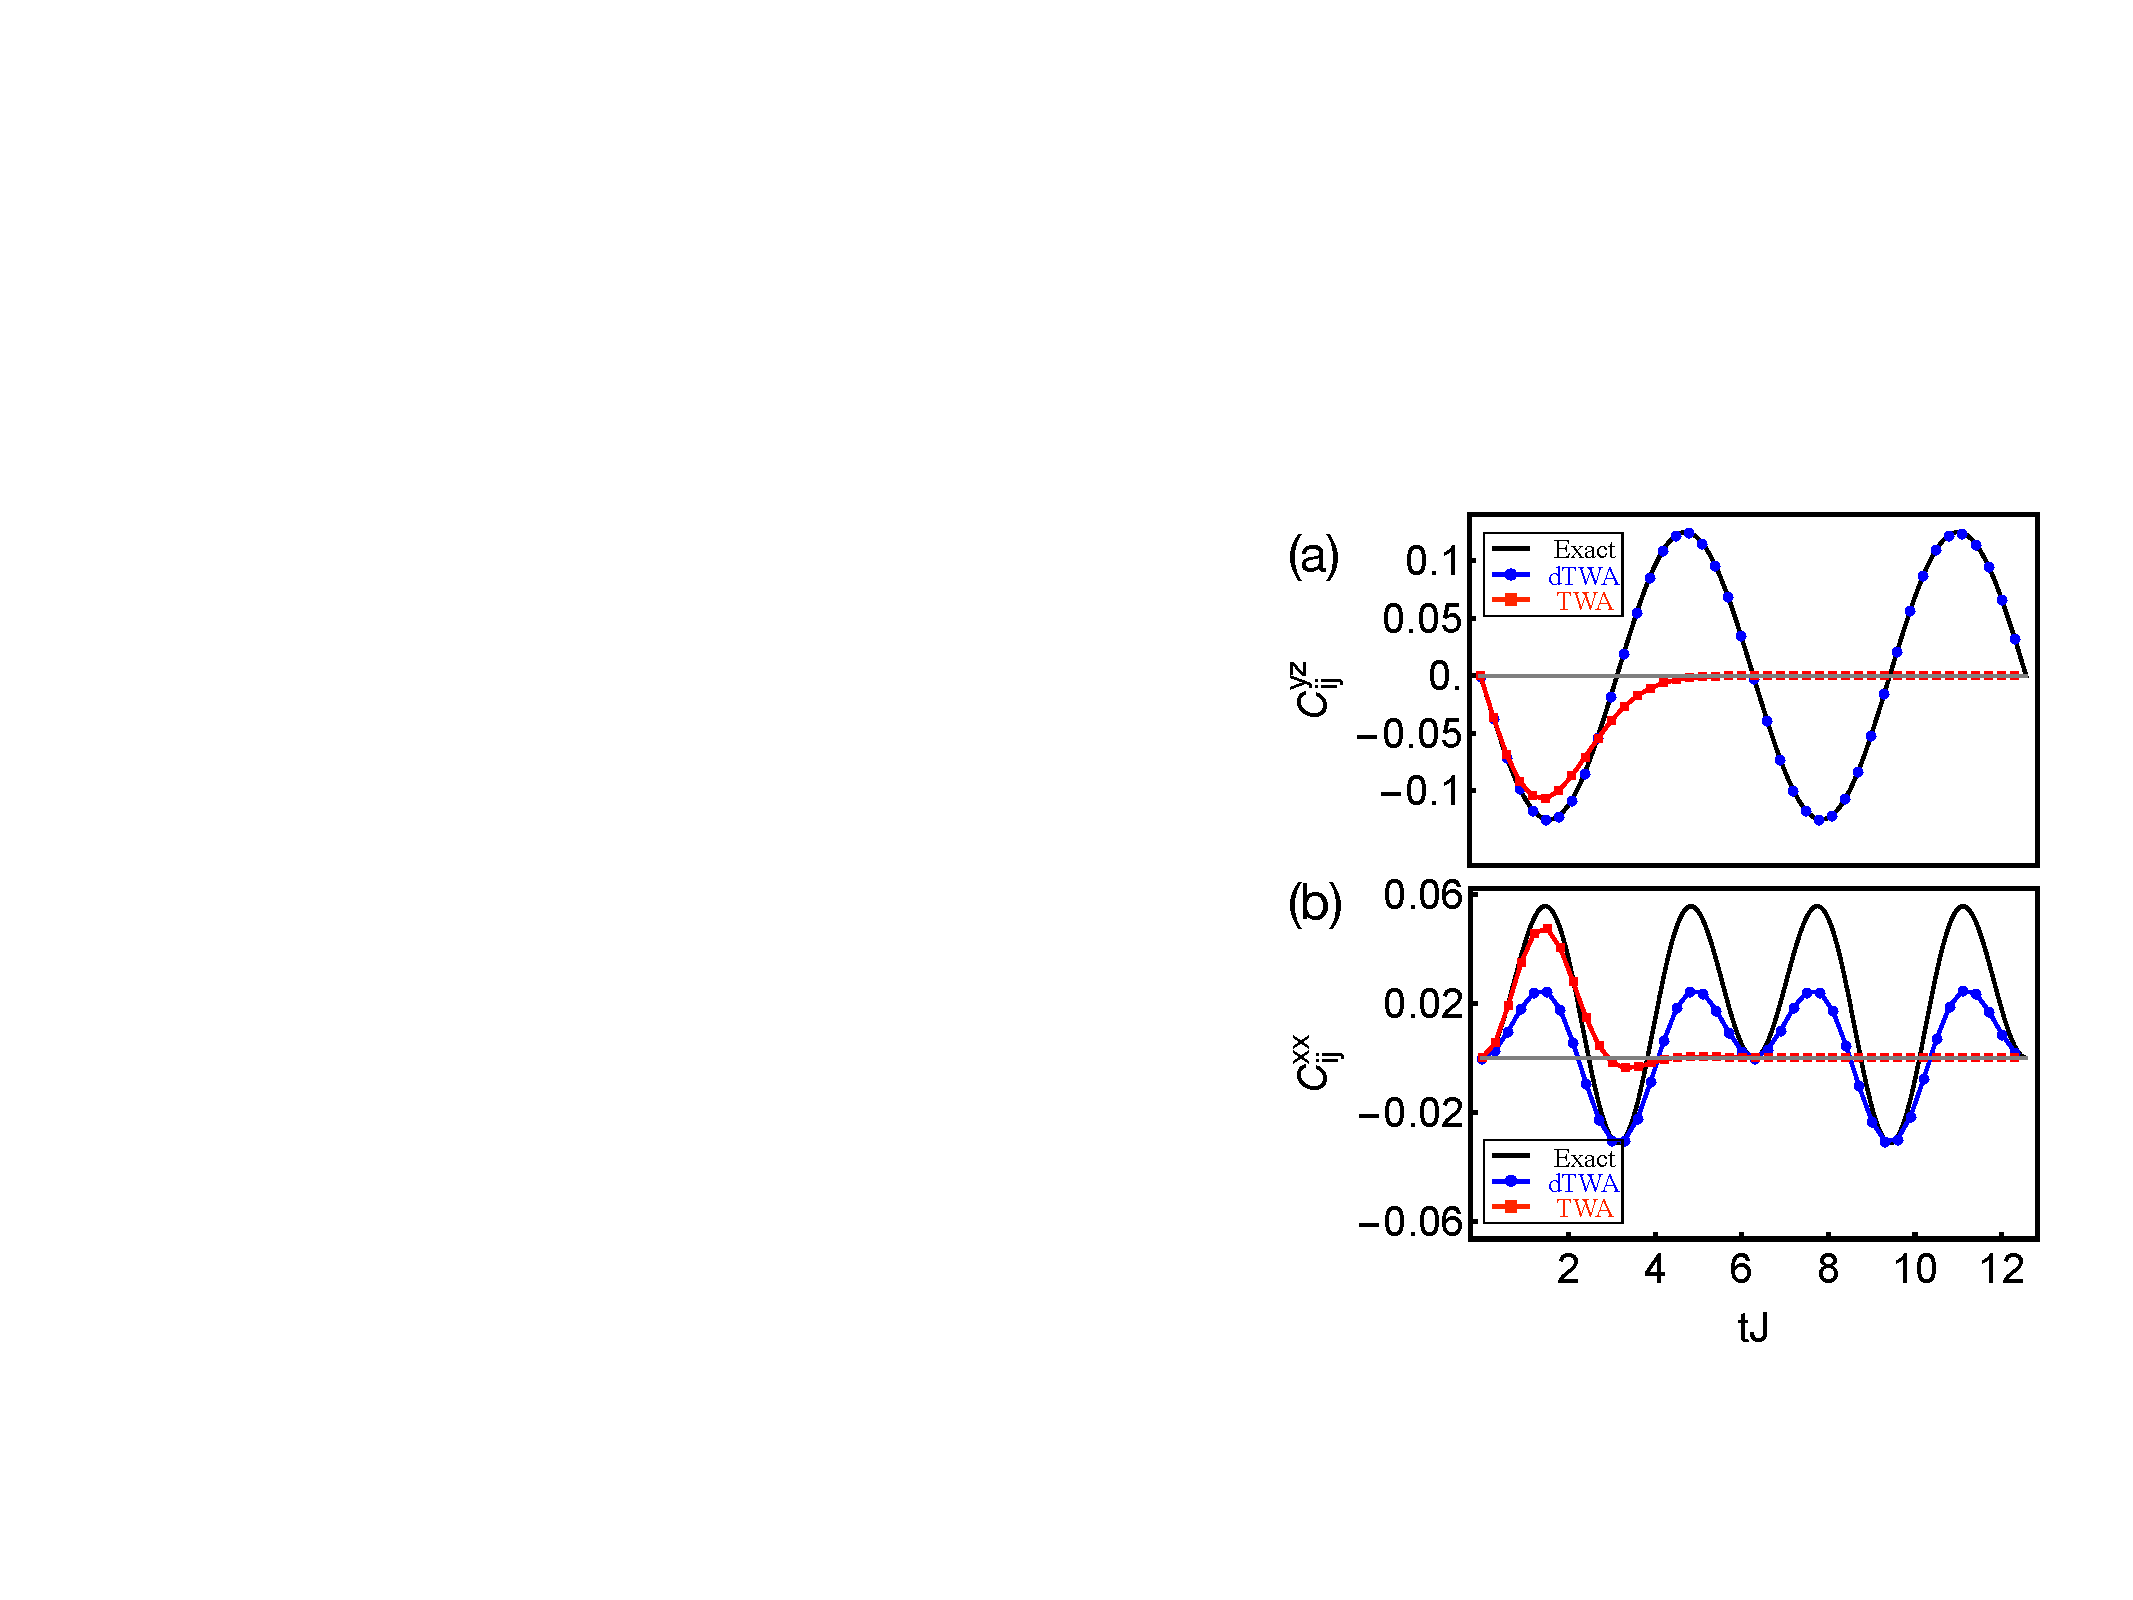
\includegraphics[width = 0.7\columnwidth]{fig1v2.pdf}
\caption{(Color online) Dynamics of one component of the spin-spin correlations for the 1D Ising model with no transverse field [Eq.~\eqref{eqn: Hising}], obtained from the exact solution (solid black), dTWA (blue circles), and TWA (red squares). (a) $C_{ij}^{yz}$ for an initial state with all spins along $\hat x$, and (b) $C_{ij}^{xx}$ for an initial state with all spins $45^\circ$ between $\hat x$ and $\hat z$. $C^{\mu\nu}_{ij}$ is defined in Eq.~\eqref{eqn: C}. The black and blue curves overlap in (a).}
\label{fig: correlation2}
\end{figure}

The key finding in this paper is that the accuracy of dTWA versus TWA is more nuanced than simply one being better than the other. We provide insight into the nature of Wigner approximations, finding commonalities in how both TWA and dTWA approximate the correlations. These insights are not readily apparent from looking at plots of the nine Cartesian components of spin-spin correlations. We are able to gain insight into the workings of TWA and dTWA and isolate the nuanced differences between them by utilizing the correlation matrix visualization (CMV) technique, which was recently introduced in Ref.~\cite{mukherjee2018geometric} building on geometrical visualization techniques in Refs.~\cite{kimura2003bloch, byrd2003characterization, jakobczyk2001geometry, tilma2002parametrization, rundle2017simple, bertlmann2008bloch, giraud2015tensor, jevtic2014quantum, dunkl2011numerical, kurzynski2016three, sorensen1984product, halstead1984multipole, donne1997pictorial, philp2005way, merkel2008quantum, dowling1994wigner, harland2012towards, gamel2016entangled, garon2015visualizing, leiner2017wigner}. CMVs encode all the information contained in spin-spin correlations into three dimensional shapes, and allow us to compare all components of the spin-spin correlations on equal footing

This article is organized as follows. In Sec.~\ref{sec: Wigner}, we introduce TWA and dTWA. In Sec.~\ref{sec: CMV}, we define CMVs. In Sec.~\ref{sec: Ising}, we use CMVs to visualize and compare spin-spin correlation dynamics for the exact solution, dTWA, and TWA applied to the 1D Ising model with no transverse field. In Sec.~\ref{sec: other}, we use CMVs to visualize and compare spin-spin correlation dynamics calculated with these three methods for the 1D transverse Ising and XX models. We distill the lessons of these comparisons and conclude in Sec.~\ref{sec: conclusions}.

\section{Wigner approximations}\label{sec: Wigner}
Wigner approximations approximate the dynamics of a system starting in an initial state $\ket{\psi(0)}$. The approximation has three steps, schematically illustrated in Fig.~\ref{fig: wigner2}. 

In the first step, we sample phase space coordinates from the Wigner function associated with the initial density matrix $\hat{\rho}(0) = \ket{\psi(0)}\bra{\psi(0)}$. The Wigner function, denoted $W(\mathbf{S})$, is a quasiprobability distribution that represents $\hat{\rho}(0)$ in an appropriate phase space, with phase points described by coordinates $\mathbf{S}$. $W(\mathbf{S})$ is defined via
\begin{equation}
\hat{\rho} = \int\! d\mathbf{S}~W(\mathbf{S}) \hat{A}(\mathbf{S}), \label{eqn: W}
\end{equation}
where $\hat{A}$ is called a phase-point operator, and the integral runs over all of phase space. The phase space coordinates that describe motional degrees of freedom are position and momentum. For spins, the coordinates can be the spin vector elements $(S^x, S^y, S^z)$. (For spins, the choice of phase space is not unique, and possible phase spaces are discussed in Secs.~\ref{subsec: TWA} and~\ref{subsec: dTWA}).

In the second step, we evolve the sampled initial phase space points in time according to classical equations for the spins. The equations of motion for the specific models we consider [Eqs.~\eqref{eqn: Hising},~\eqref{eqn: HtransIsing}, and~\eqref{eqn: HXX}] are given in Eqs.~\eqref{eqn: IsingEOM},~\eqref{eqn: transIsingEOM}, and~\eqref{eqn: XXEOM} respectively. We denote the classical trajectory of an initial point $\mathbf{S}$ by $\mathbf{S}_{\rm cl}(\mathbf{S},t)$.

In the third and final step of the approximations, we calculate the expectation of an operator $\hat{O}$ at time $t$ by averaging over the trajectories of the phase points as
\begin{equation}\label{eqn: O}
\smallexpect{\hat{O}} = \int\! d\mathbf{S}~{\rm wl}(\hat{O},\mathbf{S}_{\rm cl}(\mathbf{S},t)) W(\mathbf{S}).
\end{equation}
Here, ${\rm wl}(\hat{O},\mathbf{S})$ is the Weyl symbol for $\hat{O}$ at the phase point $\mathbf{S}$. As examples, ${\rm wl}(\hS^\mu_i,\mathbf{S}) = S^\mu_i$ and ${\rm wl}(\hS^\mu_i\hS^\nu_j+\hS^\nu_j\hS^\mu_i,\mathbf{S}) = S^\mu_iS^\nu_j+S^\nu_iS^\mu_j$. The procedure to obtain the Weyl symbol for other observables is more involved~\cite{polkovnikov2010phase}, but in this paper, we only need the examples listed here.

\begin{figure}[t]\centering
 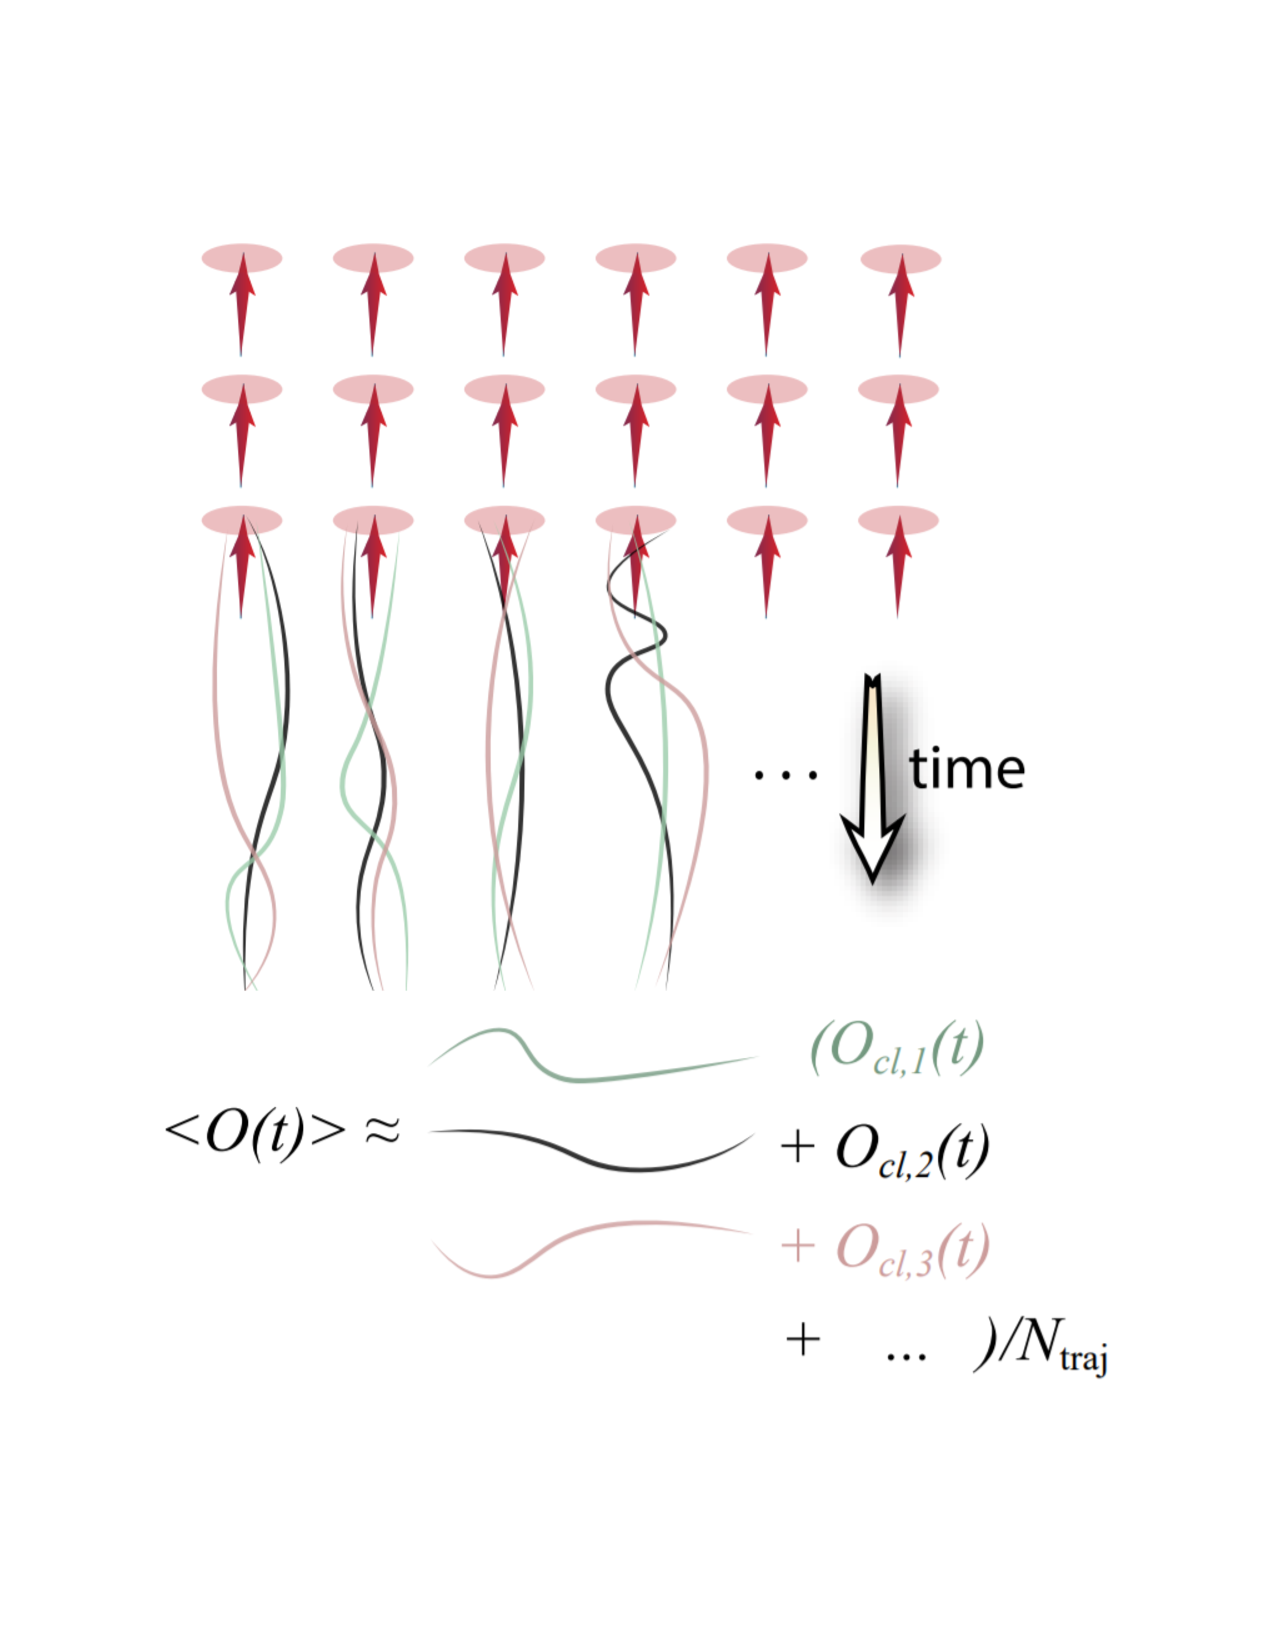
\includegraphics[width = 0.7\columnwidth]{wigner2.pdf}
 \caption{(Color online) Illustration of Wigner approximations. The approximations work in three steps: a) randomly sample points in phase space from the Wigner distribution for the initial state, b) evolve the phase points classically through time, and c) calculate the desired observable from the ensemble average of the observable at time $t$, evaluated from the time-evolved classical trajectories of the initial phase space points.}
 \label{fig: wigner2}
\end{figure}

Different Wigner approximations for spin systems differ in their choice of phase space. In this article, we focus on two kinds of approximations with two different kinds of phase spaces: TWA samples from a finite continuous area of phase space, and dTWA samples from a discrete set of phase points. We describe these schemes below.

\subsection{TWA}\label{subsec: TWA}
In the (continuous) TWA~\cite{wootters1987wigner, polkovnikov2010phase}, we map a system of $N$ spins to a product of Fock states of two bosonic fields, $\ket{\psi} = \ket{\alpha}\otimes\ket{\beta}$, where $\alpha$ and $\beta$ satisfy $|\alpha|^2+|\beta^2|=N$ and $|\alpha|^2-|\beta^2|=2\sum_i\smallexpect{\hS^z_i}$. The Wigner function for the bosonic fields is 
\begin{equation}
W(\alpha,\alpha^*,\beta,\beta^*) = 2e^{-2|\alpha|^2-2|\beta|^2}L_{N+1}\left(4|\alpha|^2\right), \label{eqn: W_alphabeta}
\end{equation}
where $L_n(x)$ is the Laguerre polynomial of order $n$.

When all the spins point along the $z$ direction, we have $|\alpha|^2=N$ and $\beta=0$. Substituting these values in Eq.~\eqref{eqn: W_alphabeta} and assuming $N\gg1$, the Wigner function can be rewritten in terms of spin coordinates in a simple manner:
\begin{equation}
W(\mathbf{S}_{\rm tot}) \approx \frac{2}{\pi N}{\rm exp}\left(-\frac{(S^x_{\rm tot})^2+(S^y_{\rm tot})^2}{N/2}\right)\delta\left(S^z_{\rm tot}-N/2\right), \label{eqn: W_TWATot}
\end{equation}
where $S^\mu_{\rm tot} = \sum_i S^\mu_i$. Then, the Wigner function for a single spin can be taken to be
\begin{equation}
W(\mathbf{S}_i) \approx \frac{2}{\pi}e^{-2(S^x_i)^2-2(S^y_i)^2}\delta\left(S^z_i-1/2\right). \label{eqn: W_TWA}
\end{equation}
We refer the reader interested in the derivation of Eqs.~\eqref{eqn: W_alphabeta} and~\eqref{eqn: W_TWATot} to Ref.~\cite{polkovnikov2010phase}.

When the system has spins all uniformly pointing along a direction besides $\hat{z}$ at the initial time, we first initialize the spins along $\hat{z}$ by sampling from Eq.~\eqref{eqn: W_TWA}, and then rotate all the spins. We always assume that the spins initially point in the $x$-$z$ plane.
This involves no loss of generality since the Hamiltonians we consider are symmetric under rotations about $\hat z$.

\subsection{dTWA}\label{subsec: dTWA}
In dTWA~\cite{schachenmayer2015many, schachenmayer2015dynamics}, the initial phase space is chosen to be a discrete set of points $\vec{\alpha}=(\vec{\alpha}_1,\vec{\alpha}_2,..\vec{\alpha}_N)$, where $\vec{\alpha}_i$ is the spin 3-vector for the $i^{\rm th}$ spin. As a result, the continuous integral in Eq.~\eqref{eqn: O} is replaced by the sum
\begin{equation}
\expect{O}(t) = \sum_{\vec \alpha}~{\rm wl}(\hat{O},\vec{\alpha}_{\rm cl}(\vec\alpha,t))W_{\vec \alpha},
\end{equation}
with $\vec{\alpha}_{\rm cl}(\vec\alpha,t)$ the classical trajectory of the initial phase point $\vec\alpha$.

The discrete locations where the initial points $\vec{\alpha}_i$ can lie are non-unique, and different works in the literature have made different choices. For example, Ref.~\cite{schachenmayer2015many} describes the case where the phase space for each spin consists of eight points given by
\begin{align}\label{eqn: S8_alpha}
&\mathbf{S}_1 = \frac{1}{2}(1,1,1),\nonumber\\
&\mathbf{S}_2 = \frac{1}{2}(-1,-1,1),\nonumber\\
&\mathbf{S}_3 = \frac{1}{2}(1,-1,-1),\nonumber\\
&\mathbf{S}_4 = \frac{1}{2}(-1,1,-1),\nonumber\\
&\mathbf{S}_{4+r} = -\mathbf{S}_r\ (1\leq r\leq4).
\end{align}
The phase point operators are defined as $\hat{A}_{\vec{\alpha}_i} = \frac{1}{2}+\vec{\alpha}_i\cdot\hat{\vec{\sigma}}$, where $\hat{\vec{\sigma}}=(\hat{\sigma}^x,\hat{\sigma}^y,\hat{\sigma}^z)$ is the vector of Pauli matrices $\hat{\sigma}^\mu$ ($\mu=x,y,z$). The phase point operator for $N$ spins is the product $\hat{A}_{\vec\alpha} = \Pi_i \hat{A}_{\vec{\alpha}_i}$. The Wigner function at $\vec{\alpha}$ is $W_{\vec \alpha} = \frac{1}{2^N}{\rm Tr}(\hat{\rho}\hat{A}_{\vec{\alpha}})$.

There is flexibility to choose other discrete sets of points in dTWA. Some of these choices are described in Ref.~\cite{pucci2016simulation}. The dynamics of spin systems sampled from different discrete phase spaces differ, as explored in detail in Ref.~\cite{pucci2016simulation}. While the phase spaces chosen in Ref.~\cite{pucci2016simulation} and other references work well for the models and initial conditions studied there, we find that those phase spaces yield significantly worse results for some of the models and conditions we consider in this paper. Therefore, we use only the phase space comprised of the phase points defined in Eq.~\eqref{eqn: S8_alpha}. For this phase space, the correlations in dTWA are accurate at small times, although as we explain later, differences from the exact dynamics appear at longer times. We have not explored the question of finding the optimal phase space that will most accurately approximate the dynamics in our study.

\section{Visualizing the correlation matrix}\label{sec: CMV}
The connected correlations between a pair of spins $i$ and $j$ are
\begin{equation}
c_{ij}^{\mu\nu} = \expect{\hS_i^\mu \hS_j^\nu}-\expect{\hS_i^\mu}\expect{\hS_j^\nu},\ \mu,\nu\in\{x,y,z\}
\end{equation}
We define their symmetric part as
\begin{equation}
C_{ij}^{\mu\nu} = \frac{c_{ij}^{\mu\nu} + c_{ij}^{\nu\mu}}{2}.\label{eqn: C}
\end{equation}
We then define a one-to-one mapping between this symmetric correlation matrix and a function proportional to a homogeneous quadratic polynomial,
\begin{equation}
Q_{ij}(\mathbf{r}) = \frac{\mathbf{r}^T\cdot C_{ij}\cdot\mathbf{r}}{(1+r^2)^{3/2}},
\end{equation}
where $\mathbf{r}$ is a $3$-vector. The CMV is the three-dimensional locus of points where $Q_{ij}(\mathbf{r})$ has a constant magnitude, i.e the set of points $\mathbf{r}$ where $Q_{ij}(\mathbf{r}) = \pm P$. Each sign is assigned a different color. We shade points where $Q_{ij}(\mathbf{r})>0$ as red, and points where $Q_{ij}(\mathbf{r})<0$ as blue. We chose $P=0.002$ more or less arbitrarily to produce our CMVs; Changing $P$ mainly changes the overall size of the CMVs. The factor $(1+r^2)^{3/2}$ in the denominator of $Q_{ij}(\mathbf{r})$ is chosen such that the size of the CMV is roughly proportional to the magnitude of the correlations; any other factor that increases faster than $r^2$ is also suitable.

There is a one-to-one mapping between $Q_{ij}(\mathbf{r})$ and $C_{ij}$, and therefore the CMV contains all the information about $C_{ij}$. The width of the CMV in a direction $\hat n$ (not necessarily a Cartesian direction) is roughly proportional to $\expect{(\hat{\vec{S_i}}\cdot \hat n) (\hat{\vec{S_j}}\cdot \hat n)}-\expect{\hat{\vec{S_i}}\cdot \hat n}\expect{\hat{\vec{S_i}}\cdot \hat n}$. Therefore, the lobes of the CMV point along the eigenvectors of $C_{ij}$, and the fatness of the lobes in that direction is proportional to the corresponding eigenvalue. Some examples of CMVs are given in Fig.~\ref{fig: CMV}.
\begin{figure}[t]\centering
 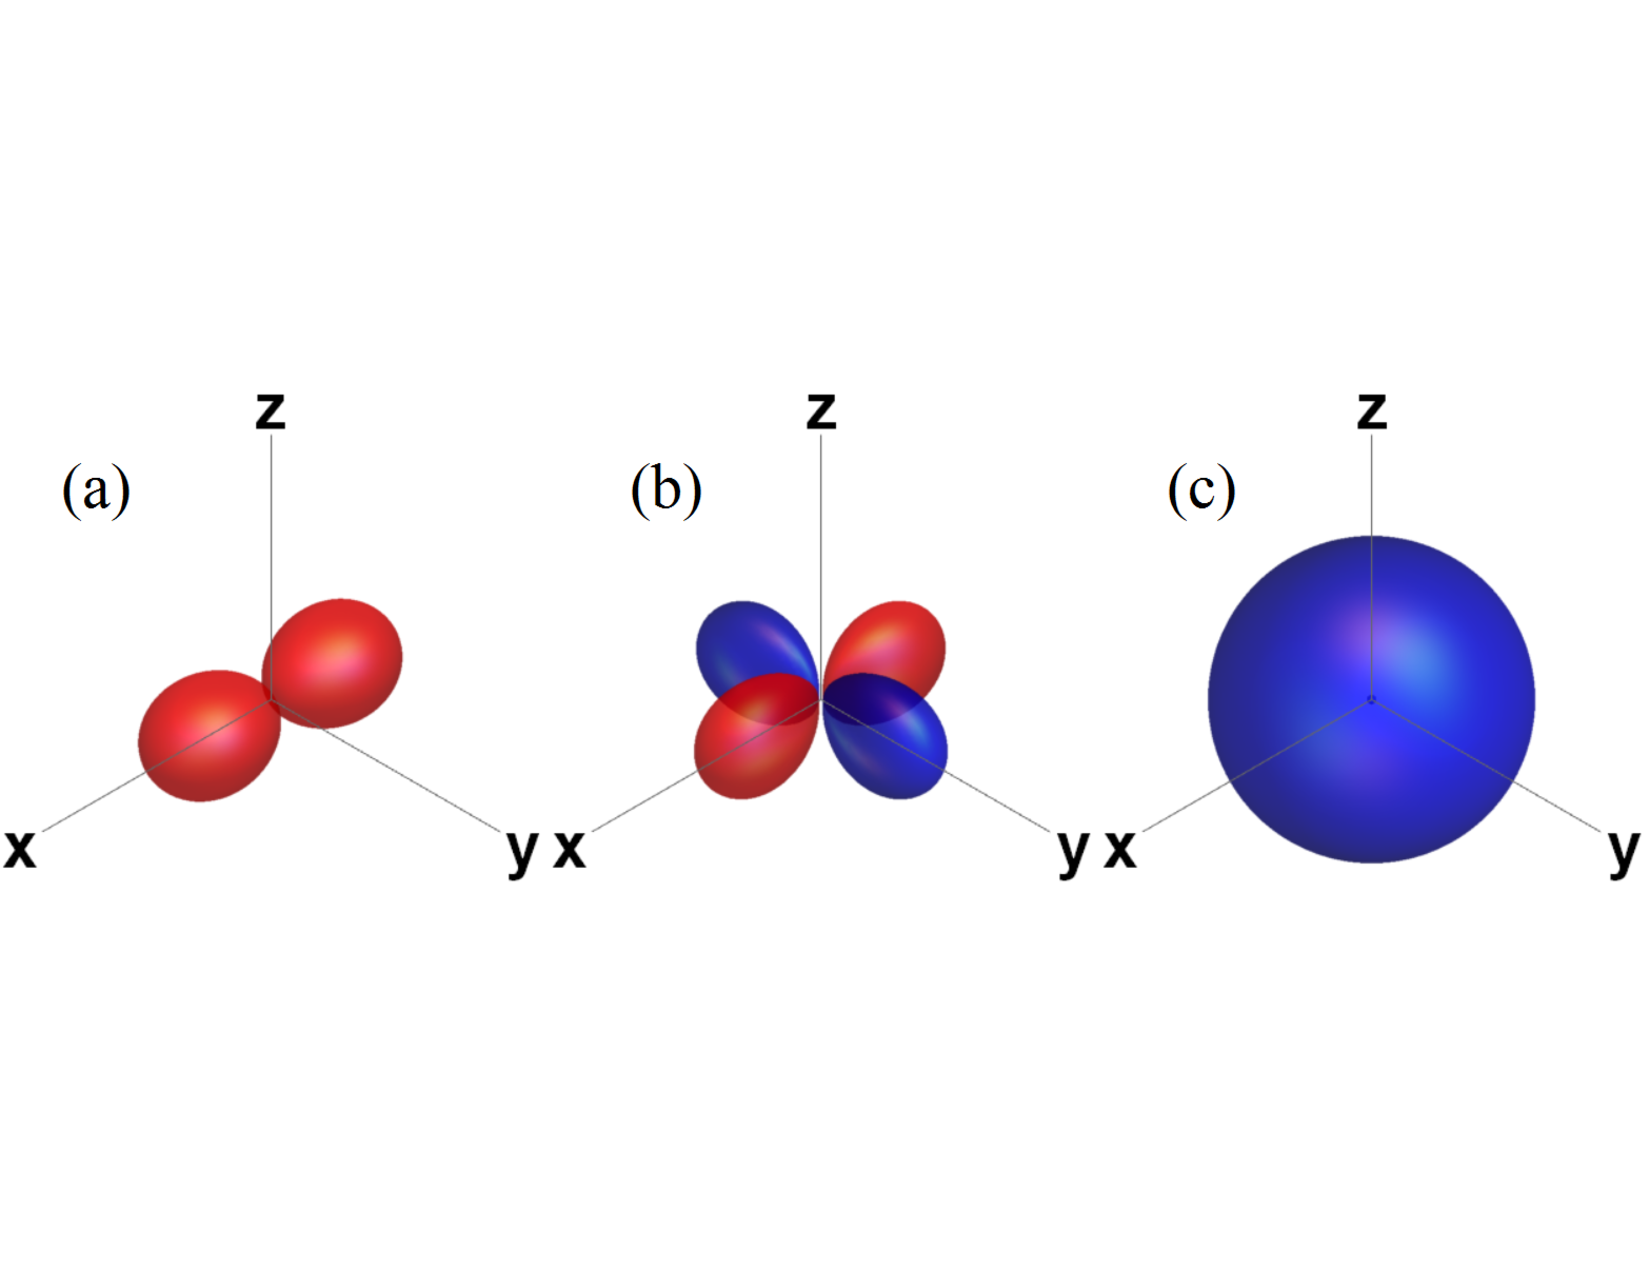
\includegraphics[width = \columnwidth]{CMV.pdf}
 \caption{(Color online) Examples of correlation matrix visualizers (CMVs). Red represents positive correlations, and blue represents negative correlations. The three panels show the CMV for a system with the correlation matrix $C_{ij}$ = $\left(\begin{array}{ccc}1/4&0&0\\0&0&0\\0&0&0\end{array}\right)$ in (a), $\left(\begin{array}{ccc}1/4&0&0\\0&-1/4&0\\0&0&0\end{array}\right)$ in (b), and $\left(\begin{array}{ccc}-1/4&0&0\\0&-1/4&0\\0&0&-1/4\end{array}\right)$ in (c). All three examples correspond to states that could occur physically.
 }
 \label{fig: CMV}
\end{figure}

We characterize spin-spin correlations via four main features of the CMV associated with those correlations. These features are the CMV's size, shape, dimensionality, and orientation. The CMV's size roughly translates to the magnitude of the eigenvalues of $C_{ij}$. The CMV's shape is related to the ratio of the three eigenvalues to each other. For example, as in Fig.~\ref{fig: CMV}(a), the CMV's shape is a dumbbell if two eigenvalues are much smaller in magnitude than the third. Other distinct shapes that may occur are clover (when one eigenvalue is much smaller in magnitude than the other two, as in Fig.~\ref{fig: CMV}(b)), spherical (when all three eigenvalues are equal and have the same sign, as in Fig.~\ref{fig: CMV}(c)), and wheel-and-axle (when two eigenvalues have the same sign and the third has an opposite sign). The CMV's dimensionality is contained in the description of its shape, but this feature is so important in our comparisons that we classify it separately. A dumbbell-shaped CMV is one-dimensional, a clover-shaped one is two-dimensional, and a sphere is three-dimensional. The CMV's orientation tells us the directions of the eigenvectors of $C_{ij}$.

We will find that the differences between the correlation dynamics in the Wigner approximations and the exact dynamics can be satisfactorily described by categorizing the differences between these four features of the respective CMVs. For example, we observe distinct and fairly simple trends such as that dTWA captures the revivals in the size of the CMVs more accurately than TWA, but the TWA always seems to capture the orientation of the CMVs at least as accurately as dTWA or better. On the other hand, the conventional way of plotting all components of the correlation matrix is cumbersome, and reveals little information about trends for the accuracy of TWA versus dTWA. \hyperref[sec: component plots]{Appendix A} show the conventional component-wise analysis of correlations for the dynamics considered in the main text, so a curious reader can explore these themselves.

We now use CMVs to compare the results of dTWA, TWA, and the exact solution for the dynamics of spin-spin correlations in the 1D Ising model with and without a transverse field, and 1D XX models, for various initial states. All our numerical integrations are performed on 1D chains with 10 spins, and we always calculate the correlations between the fifth and the sixth spin. For the times we consider, we observe no significant boundary effects. All our Wigner approximations have $10^4$ samples. For the 1D Ising model with no transverse field, the correlations used to make CMVs are calculated by analytically integrating the Ising equations [see Eq.~\eqref{eqn: IsingEOM} and \hyperref[sec: analytical_expns]{Appendix B}].

\section{1D Ising model}\label{sec: Ising}
We calculate the dynamics of nearest-neighbor correlations in a 1D Ising model:
\begin{equation}\label{eqn: Hising}
\hH_I = -\sum_i J \hS_i^z\hS_{i+1}^z,
\end{equation}
where the sum runs over neighboring pairs of spins only.
The spins satisfy the equations
\begin{align}\label{eqn: IsingEOM}
\dot{\hS}_i^x &= \hS_i^y\hB_i^z,\nonumber\\
\dot{\hS}_i^y &= -\hS_i^x\hB_i^z,\\
\dot{\hS}_i^z &= 0,\nonumber
\end{align}
where $\hB_i^\mu = J\left(\hS_{i-1}^\mu+\hS_{i+1}^\mu\right)$, and we have set $\hbar=1$. We initialize the system in $\ket{\theta\theta\theta\textellipsis}$, with
\begin{equation}
\ket{\theta}=\cos\frac{\theta}{2}\ket{\uparrow}+\sin\frac{\theta}{2}\ket{\downarrow}.
\end{equation}

First, we study the case $\theta=\pi/2$. We integrate Eq.~\eqref{eqn: IsingEOM} to obtain analytical expressions for spin-spin correlations in the exact solution, dTWA, and TWA. These solutions are presented in \hyperref[sec: analytical_expns]{Appendix B}. We calculate spin-spin correlations from these analytical results, and make CMV plots for the exact dynamics, dTWA, and TWA in Fig.~\ref{fig: Isingpi2}. We find that the shape and orientation of the CMVs are captured well by both TWA and dTWA, and the size is captured well at short times. Visually, the CMVs resemble a clover. However, both TWA and dTWA fail to capture the correlations along the direction where $C_{ij}$ has the smallest eigenvalue. This failure reflects in the two-dimensional nature of the TWA and dTWA clovers; the CMVs don't extend at all in the third dimension. As we shall see, this is a general feature of Wigner approximations in all the cases we consider. Moreover, at long times, as anticipated from looking at the components of the correlations in \hyperref[sec: analytical_expns]{Appendix B}, the CMVs in TWA exponentially shrink in size, while the CMVs in dTWA and the exact solution undergo periodic oscillations at a period somewhat longer than the longest time in Fig.~\ref{fig: Isingpi2}.
\begin{figure}[t]\centering
 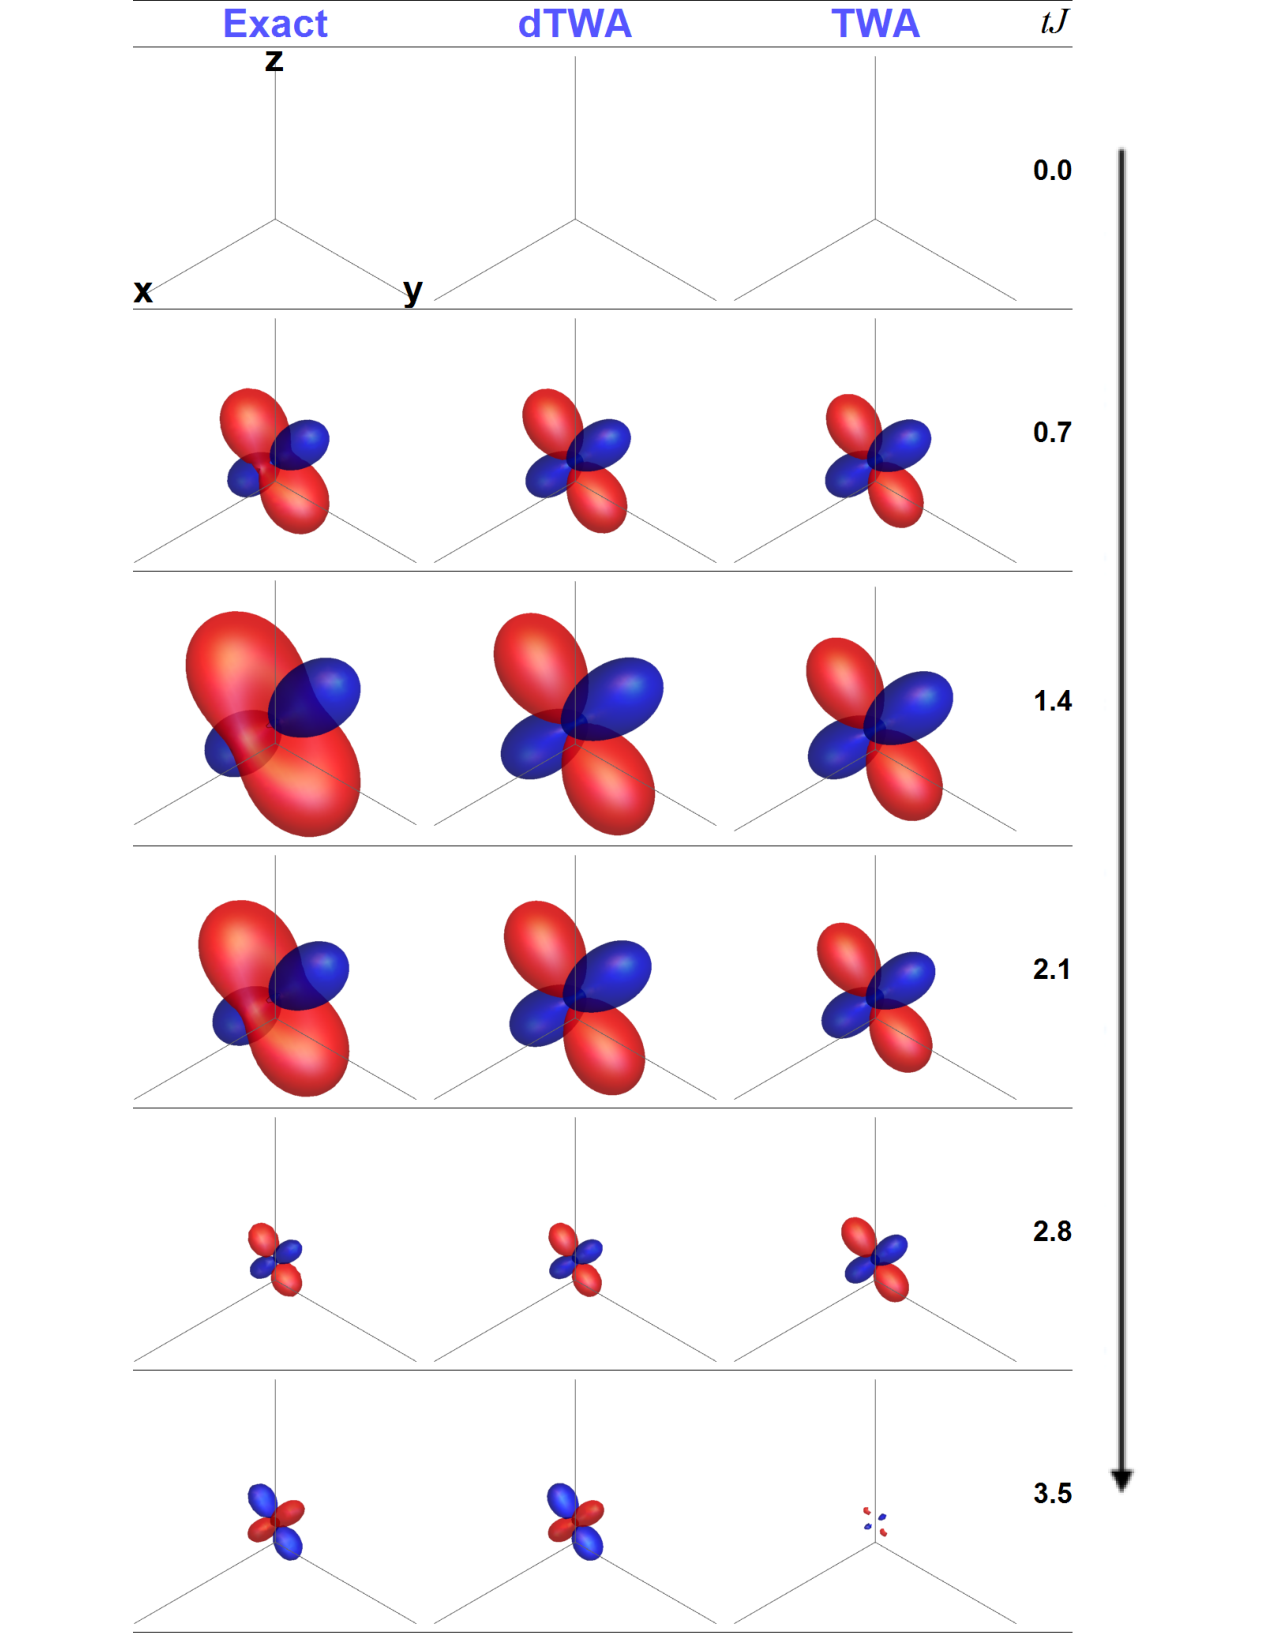
\includegraphics[width = 0.9\columnwidth]{Isingpi2modified2.pdf}
 \caption{(Color online) The CMV for nearest-neighbor spin-spin correlations at different times in the nearest-neighbor 1D Ising model in the absence of a transverse field, for the exact solution (left), dTWA (middle), and TWA (right). At $t=0$, all the spins are aligned along $\hat x$, i.e. $\theta = \frac{\pi}{2}$. An animated movie showing this dynamics is included in the Supplementary Information~\cite{supplement}.}
 \label{fig: Isingpi2}
\end{figure}
\begin{figure}[t]\centering
 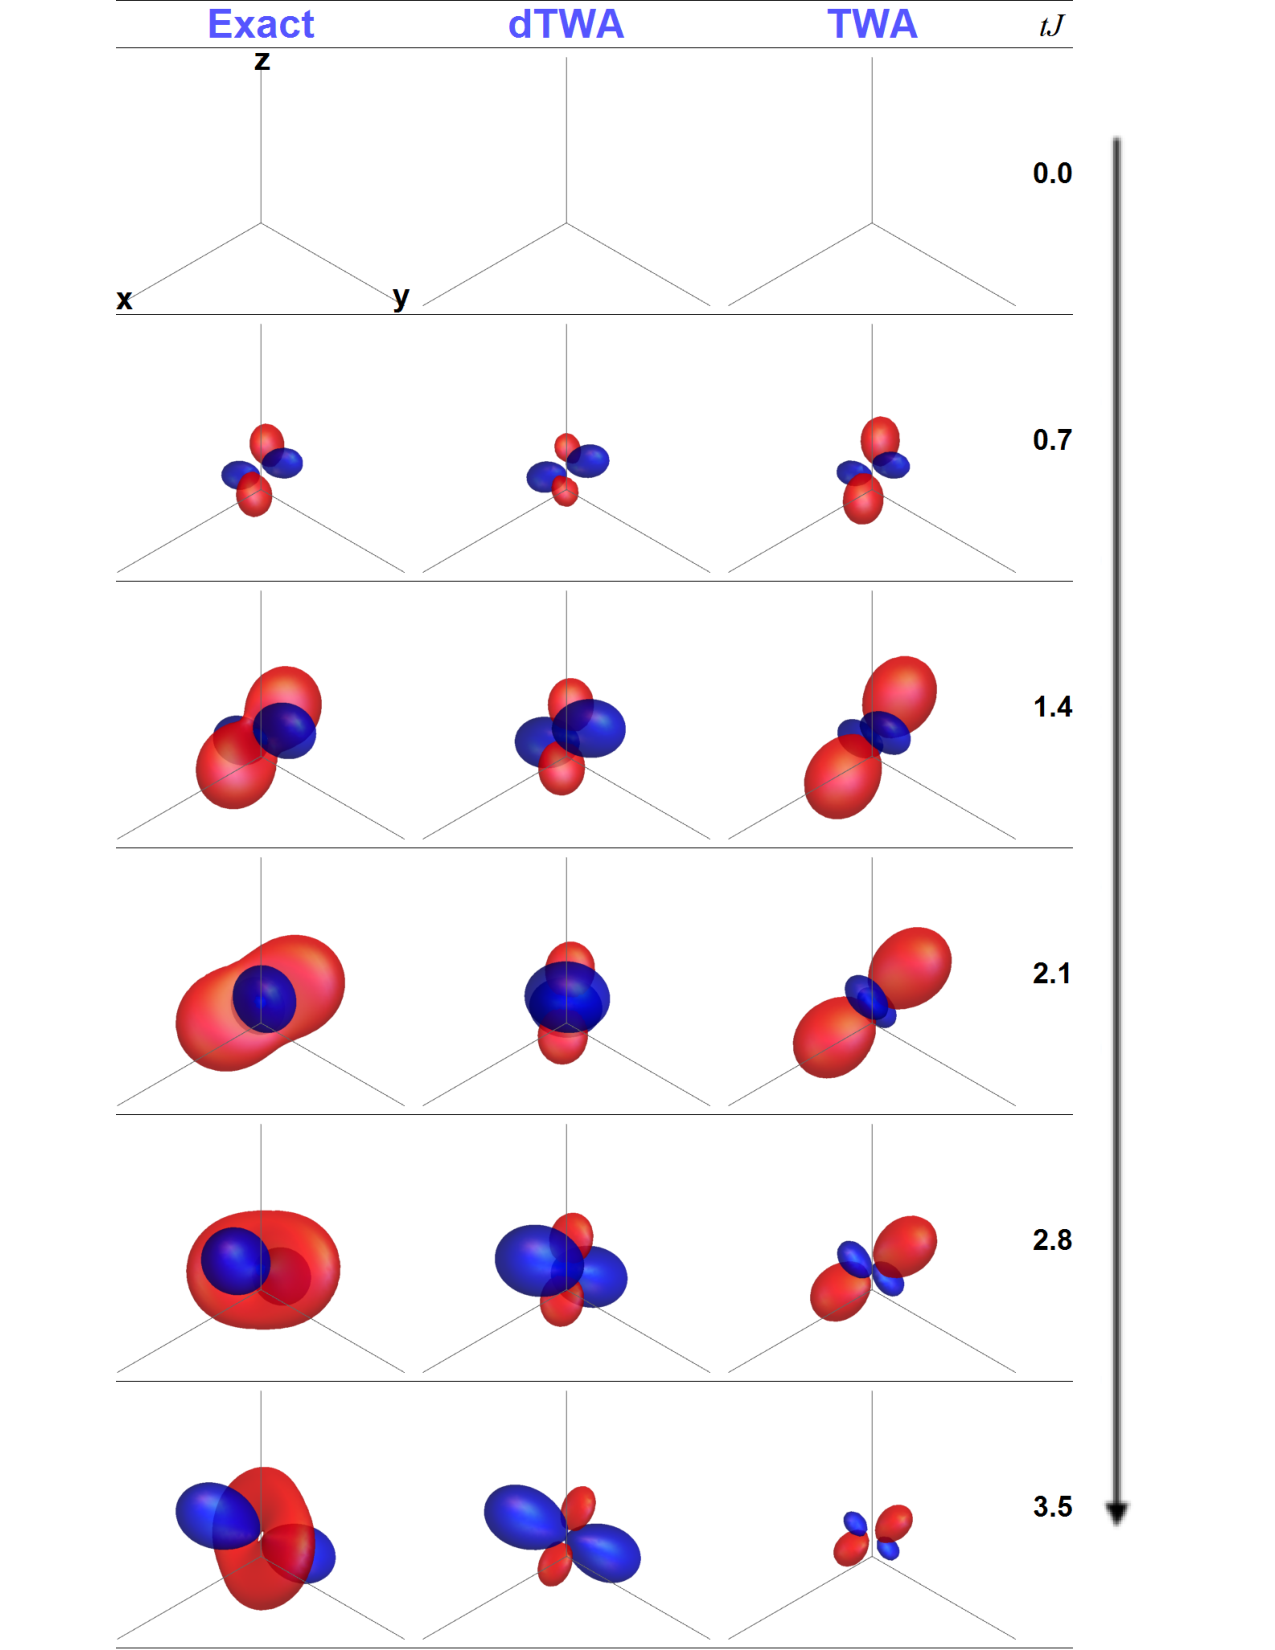
\includegraphics[width = 0.9\columnwidth]{Isingpi4modified2.pdf}
 \caption{(Color online) The CMV for nearest-neighbor spin-spin correlations at different times in the nearest-neighbor 1D Ising model in the absence of a transverse field, for the exact solution (left), dTWA (middle), and TWA (right). At $t=0$, all the spins are aligned halfway between $\hat x$ and $\hat z$, i.e. $\theta = \frac{\pi}{4}$. An animated movie showing this dynamics is included in the Supplementary Information~\cite{supplement}.}
 \label{fig: Isingpi4}
\end{figure}
\begin{figure}[t]\centering
 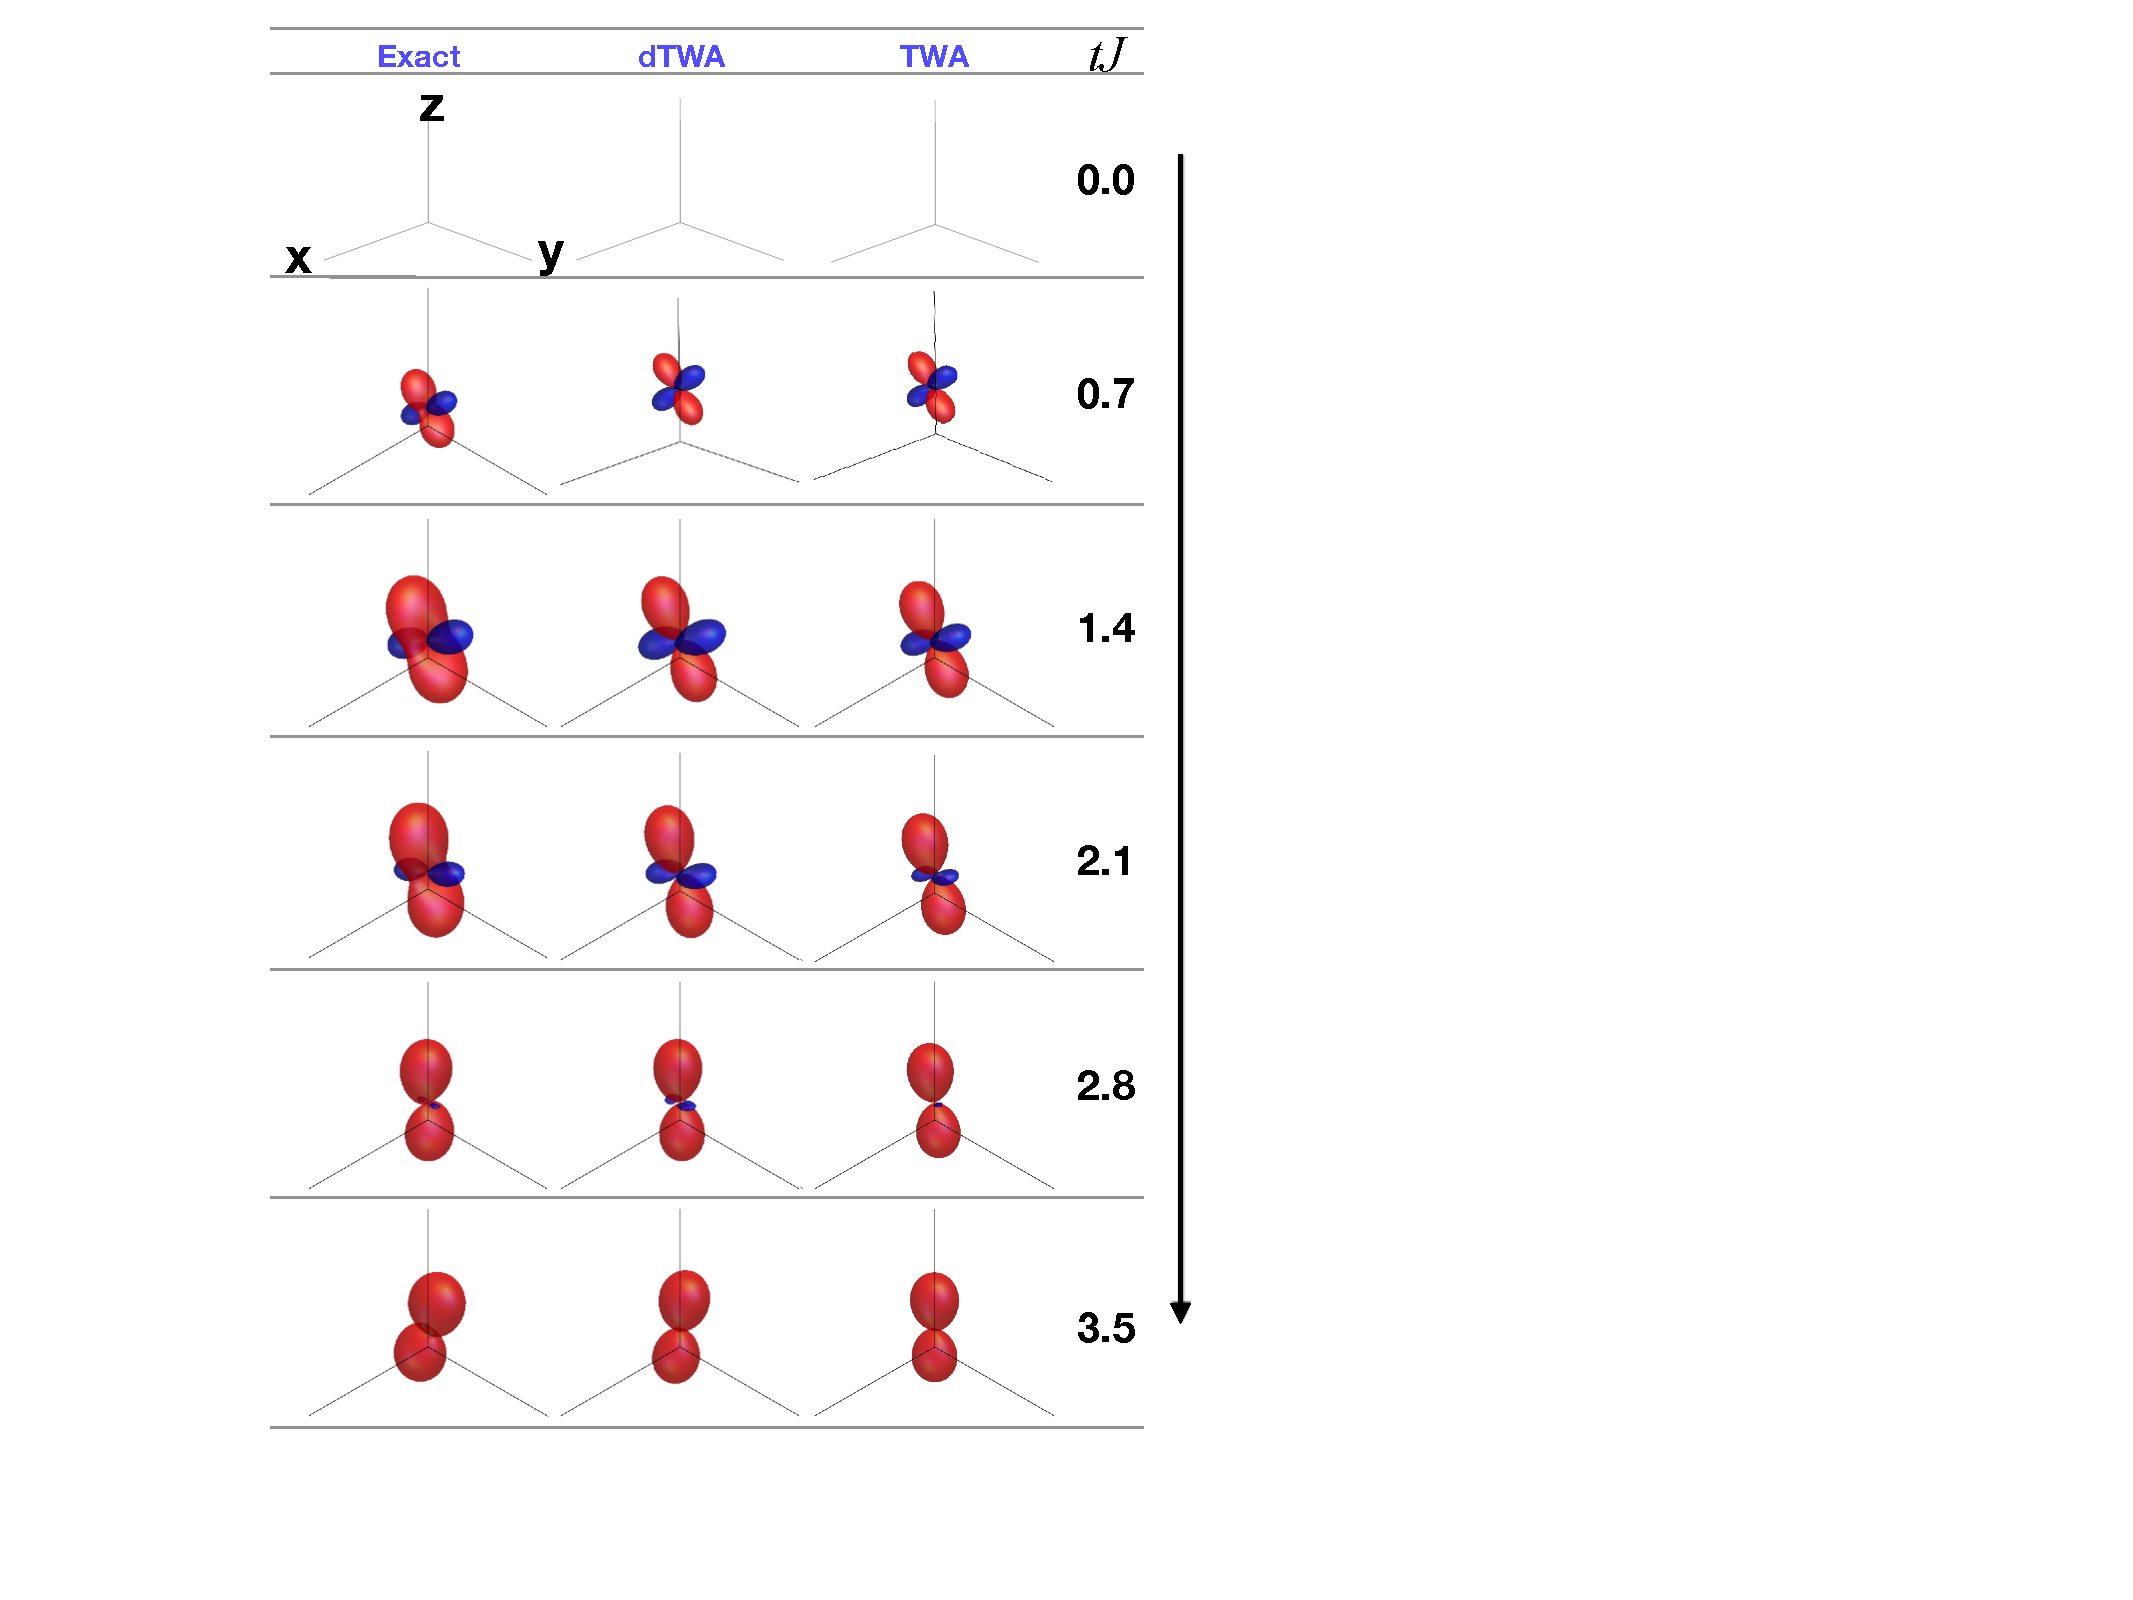
\includegraphics[width = \columnwidth]{fig6small.pdf}
 \caption{(Color online) The CMV for nearest-neighbor spin-spin correlations in a nearest-neighbor 1D transverse Ising ($h=J/3$) system at different times, for the exact solution (left), dTWA (middle), and TWA (right). At $t=0$, all the spins are aligned along $\hat x$, i.e. $\theta = \frac{\pi}{2}$. An animated movie showing this dynamics is included in the Supplementary Information~\cite{supplement}.}
 \label{fig: transIsing}
\end{figure}
\begin{figure}[t]\centering
 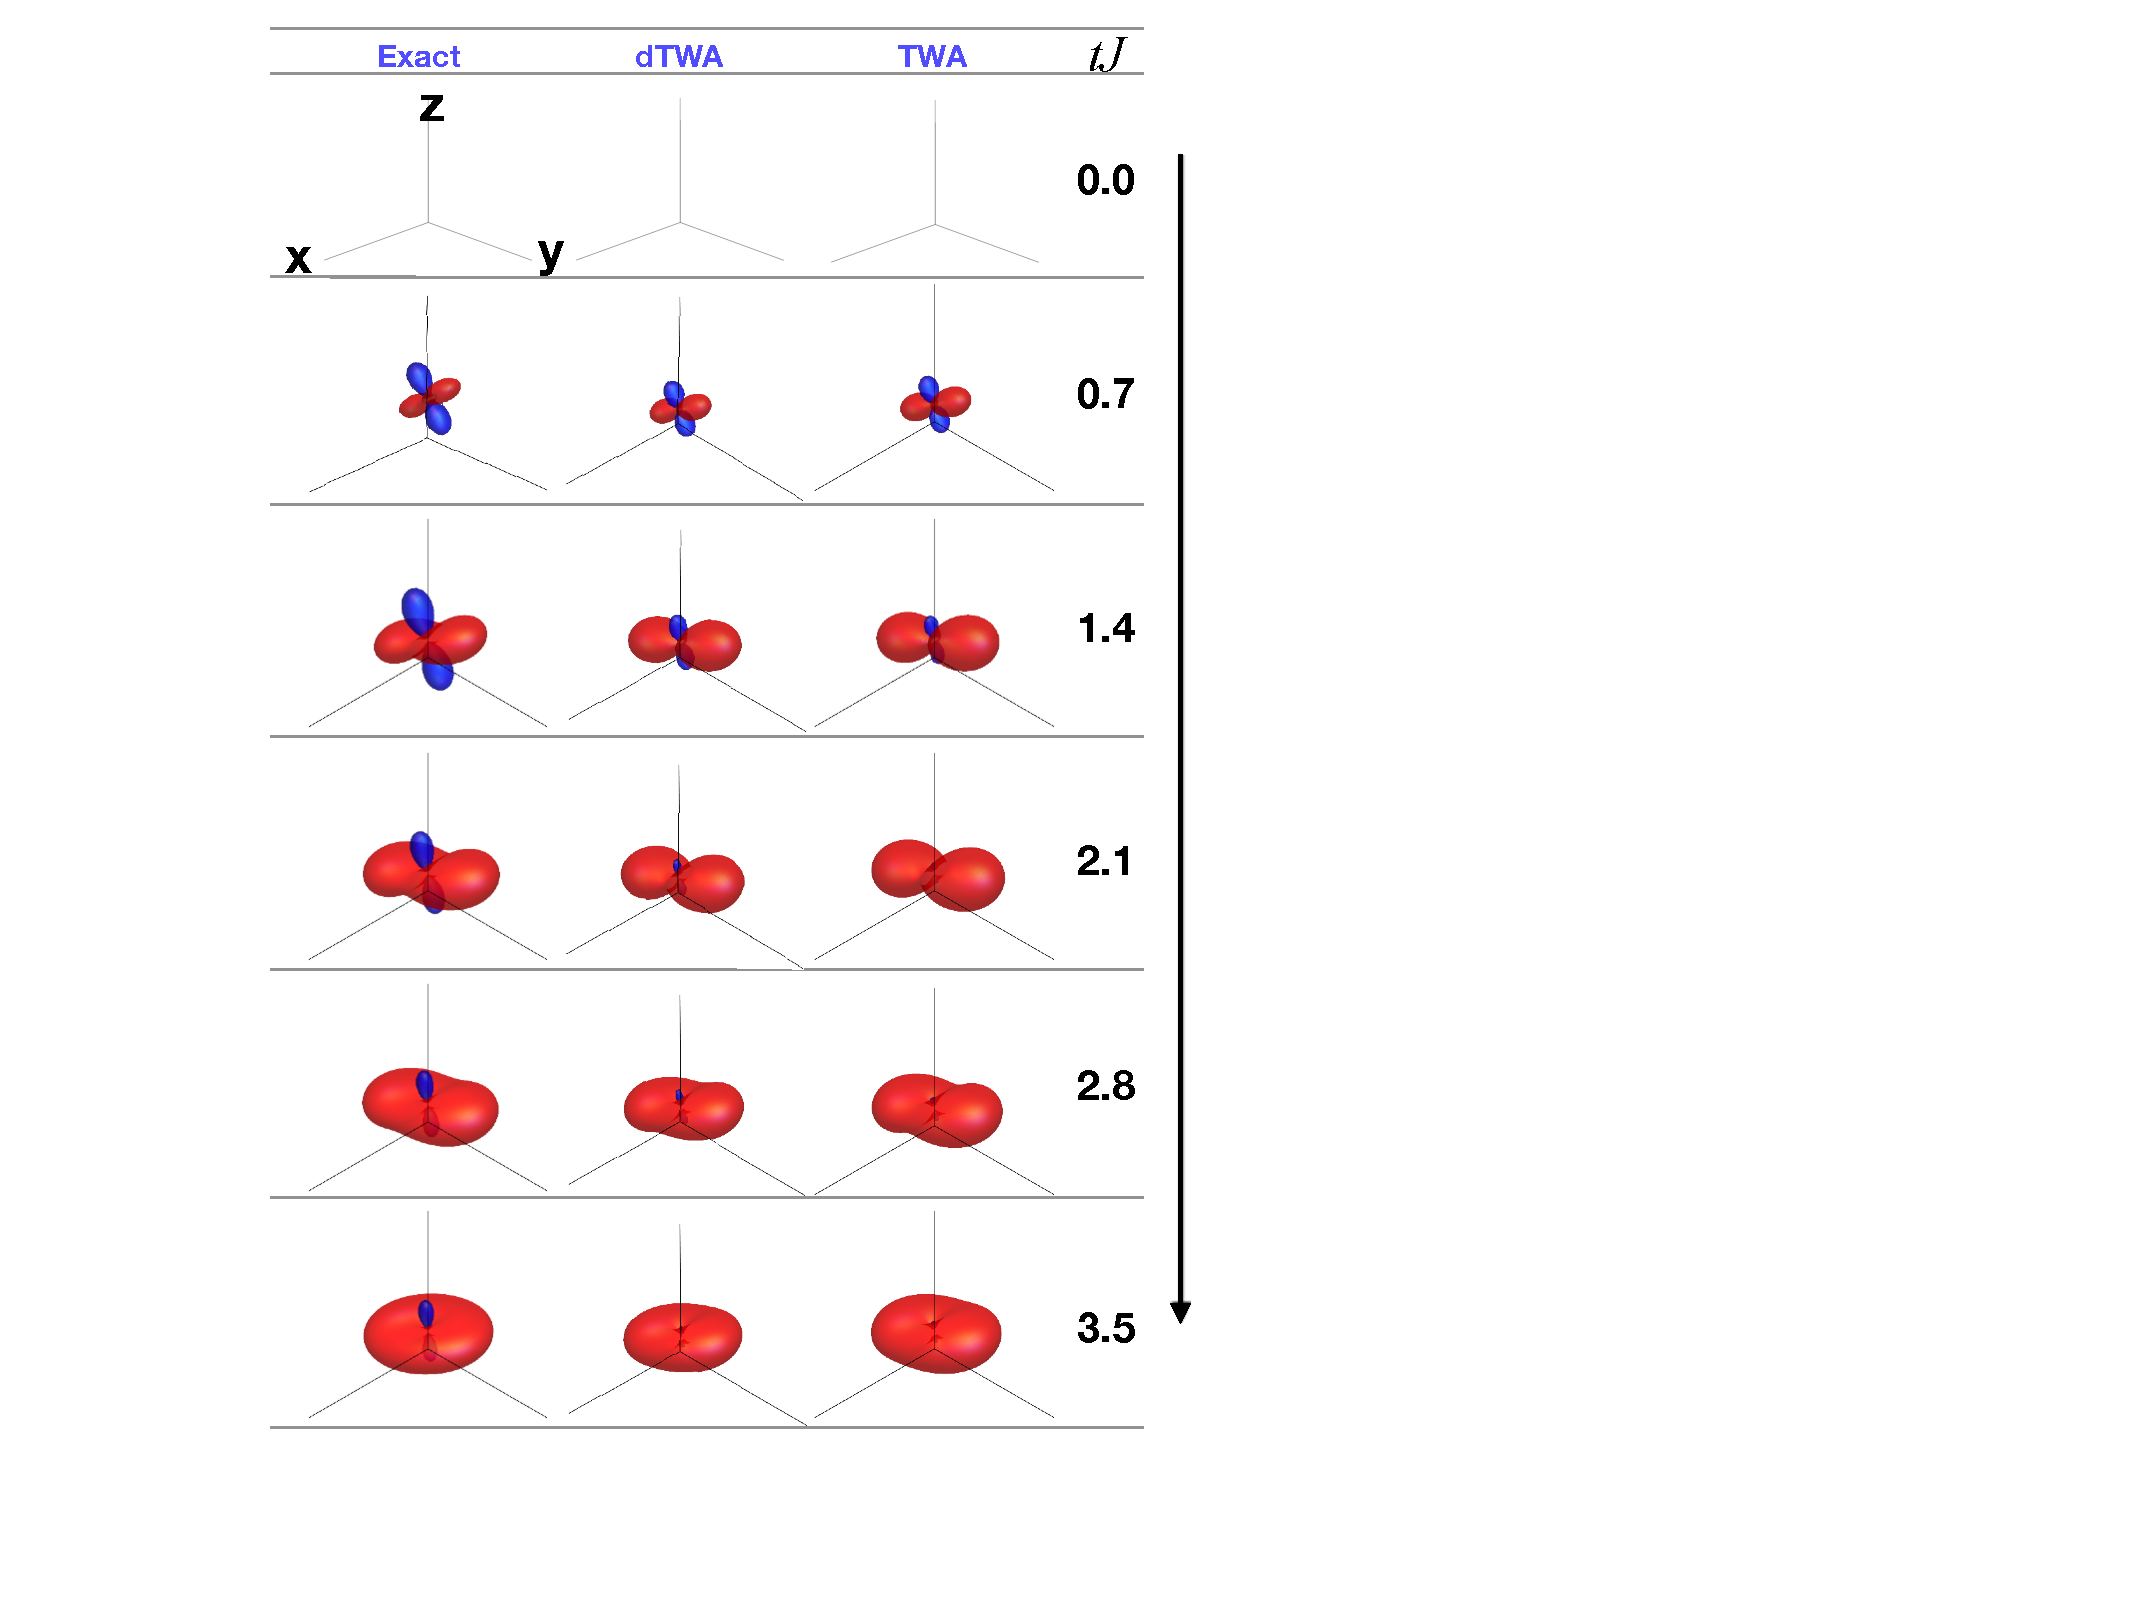
\includegraphics[width = \columnwidth]{fig7small.pdf}
 \caption{(Color online) The CMV for nearest-neighbor spin-spin correlations in a 1D system with an $XX$ Hamiltonian, calculated for the exact solution (left), dTWA (middle), and TWA (right), at different times. At $t=0$, all the spins are aligned along $\hat x$, i.e. $\theta = \frac{\pi}{2}$. An animated movie showing this dynamics is included in the Supplementary Information~\cite{supplement}.}
 \label{fig: XX}
\end{figure}

The inaccuracies of dTWA and TWA for the initial state $\ket{\theta=\pi/2}$, which are readily visible in the CMVs in Fig.~\ref{fig: Isingpi2}, may be missed when plotting specific correlation components, as is the case with Fig.~\ref{fig: correlation2}(a), which plots $C^{yz}_{ij}$ versus time. This component can be viewed as a slice of the CMVs in Fig.~\ref{fig: Isingpi2} along $\frac{\hat{y}+\hat{z}}{\sqrt{2}}$, because $C^{yy}_{ij}$ and $C^{zz}_{ij}$ are zero at all times in all the three methods for the initial state $\theta=\pi/2$. While Fig.~\ref{fig: correlation2}(a) does convey that the dynamics of $C^{yz}_{ij}$ are captured correctly at all times by dTWA and at short times by TWA, the CMVs in Fig.~\ref{fig: Isingpi2} efficiently present a much more complete picture: the approximations correctly capture correlations along all directions on the $y$-$z$ plane, but completely miss correlations along $\hat{x}$. In this case, the missing pieces would be clearly shown by plotting all Cartesian components of the correlations [see Fig.~\ref{appendix1}]. However, such behavior is far less apparent for other models or initial conditions, as we will see in the following sections. The reason is that the direction misrepresented by the Wigner approximations is often not aligned along a Cartesian direction.

Wigner approximations are less accurate for initial states different from $\theta=\pi/2$. Figure~\ref{fig: Isingpi4} depicts the CMVs for the correlations in the exact solution, dTWA, and TWA, when the initial state has $\theta=\pi/4$. 
The CMVs in both Wigner approximations are again two-dimensional at all times. Aside from the two-dimensionality, the shape of the CMVs in the Wigner approximation reasonably agree with the exact solution. The orientation of the CMVs in dTWA is worse than that of TWA at the later times considered here. The CMVs in TWA exponentially shrinks in size, while the CMVs in dTWA and the exact solution undergo periodic oscillations at a period somewhat longer than the longest time presented in Fig.~\ref{fig: Isingpi4}.

The missing pieces in the Wigner approximations for the initial state $\ket{\theta=\pi/4}$ are completely obscured in the component-wise correlation plots, as can be observed in Fig.~\ref{fig: correlation2}(b), which plots $C^{xx}_{ij}$, that is the size of the CMVs along $\hat{x}$. Even when we plot all the Cartesian components [see Fig.~\ref{appendix2}], it is nearly impossible to conclude that the Wigner approximations completely miss correlations along one direction, whereas this information is readily available in Fig.~\ref{fig: Isingpi4}. This is because the missing correlation is not aligned with a Cartesian direction.

For $\theta\neq0,\pi/2$, we note that dTWA presents a serious numerical obstacle in its implementation: there is a sign problem. The sign problem is notorious in quantum Monte Carlo algorithms, where it arises in fermionic systems as a result of negative wavefunctions due to anticommutations. In dTWA, the sign problem arises because the Wigner function is negative at some of the phase space points. In these cases, we sample the initial points $\mathbf{S}$ in phase space with weights $\frac{\left|W(\mathbf{S})\right|}{\int\! d\mathbf{S}~\left|W(\mathbf{S})\right|}$, and multiply the Weyl symbol for the trajectory of $\mathbf{S}$ by the sign of $W(\mathbf{S})$. When the sign problem occurs, a larger sample size is required to obtain a precise ensemble average (i.e with a small sampling error) for any observable. For example, the sampling error for $C^{yy}_{ij}$ at $t=0$ for a sample size of $10^4$ is $0.019$. This error is comparable to the magnitude of $C^{yy}_{ij}$ during the dynamics, and therefore we do not get much useful information about the correlation dynamics. The sampling error for $C^{yy}_{ij}$ at $\theta=\pi/4$ reduces to $0.003$ for a larger sample size of $10^5$. This obstacle is not present for $\theta=\pi/2$, where the sampling error for $C^{yy}_{ij}$ for a sample size of $10^4$ is only $0.002$. Other components have similar errors for these sample sizes.

The sign problem in dTWA can be ameliorated by rotating the phase space, such that the Wigner function is always positive at the initial phase points that are sampled. However, due to the different alignment between these points and the distinguished directions in the Hamiltonian (e.g. the $z$ direction in the Ising model), the accuracy of the dTWA would need to be re-evaluated. 

\section{XX and transverse Ising models}\label{sec: other} 

For the 1D transverse Ising model given by
\begin{equation}\label{eqn: HtransIsing}
\hat{H}_{\rm T} = \hat{H}_{\rm I} - h \sum_i \hS^x_i,
\end{equation}
the spins satisfy the equations
\begin{align}\label{eqn: transIsingEOM}
&\dot{\hS}_i^x = \hS_i^y \hB_i^z\nonumber\\
&\dot{\hS}_i^y = - \hS_i^x \hB_i^z + h \hS_i^z\\
&\dot{\hS}_i^z = - h \hS_i^y.\nonumber
\end{align}
Figure~\ref{fig: transIsing} depicts the CMVs obtained from a numerical implementation of exact diagonalization, dTWA, and TWA, when the system is initialized in $\theta=\pi/2$, and evolves under the 1D transverse Ising model with $h=J/3$. The size, shape, and orientation of the CMVs in TWA and dTWA all approximately match with the exact solution, but as in the $h=0$ cases, the CMVs are two-dimensional in both approximations. All the CMVs in these dynamics precess around the magnetic field.

For the 1D XX model given by
\begin{equation}\label{eqn: HXX}
\hat{H}_{\rm XX} = - J\sum_{i} (\hS^x_i \hS^x_{i+1} + \hS^y_i \hS^y_{i+1})
\end{equation}
the spins satisfy the equations
\begin{align}\label{eqn: XXEOM}
&\dot{\hS}_i^x = - \hS_i^z \hB_i^y\nonumber\\
&\dot{\hS}_i^y = \hS_i^z \hB_i^x\\
&\dot{\hS}_i^z = \hS_i^x\hB_i^y - \hS_i^y\hB_i^x.\nonumber
\end{align}
Figure~\ref{fig: XX} depicts the CMVs obtained from a numerical implementation of exact diagonalization, dTWA, and TWA, when the system is initialized in $\theta=\pi/2$, and evolves under the 1D XX model. The size, shape, and orientation of the CMVs in TWA and dTWA all approximately match with the exact solution, but the CMVs are two-dimensional in both approximations. Interestingly, the direction along which the CMVs are squished seems to change with time somewhat independently of the CMVs' orientations: the CMVs are more squished along $\hat{x}$ for $tJ<2.1\hbar$, and they are more squished along $\hat{z}$ for $tJ>2.1\hbar$.

\begin{table}[h]\centering
\begin{tabular}{|c|c|c|c|c|c|}
\hline
Method & Size & Revivals & Shape & Dimensionality & Orientation\\
\hline
dTWA & \check & \check & \check & $\times$ All cases& $\times(\theta=\pi/4)$\\
\hline
TWA & \check & $\times$ Ising & \check & $\times$ All cases& \check\\
\hline
\end{tabular}
 \caption{A summary of the abilities of TWA and dTWA in capturing different aspects of spin-spin correlation dynamics in 1D Ising, transverse Ising, and $XX$ systems evolving from an initial product state. We categorize dTWA's and TWA's ability to correctly capture the size of CMVs at short times, revival of CMVs at longer times (if applicable), and the shape, dimensionality, and orientation of CMVs. A checkmark refers to the respective feature being captured correctly in all the conditions we considered. Any text in the cell indicates the specific case(s) where the approximation failed. In all our cases, the CMVs' size is correct at short times, and the shape is always correct except for missing the ``three-dimensionality''.}
 \label{table: conclusion}
\end{table}

\section{Conclusions}\label{sec: conclusions}
We have demonstrated that the accuracy of Wigner approximations is more nuanced than previously believed, and uncovered properties seemingly intrinsic to both TWA and dTWA, namely that they incorrectly predict suppressed correlations along one direction. This missing aspect is often difficult to catch in conventional component-wise plots due to the sheer number and complexity of the correlations, and often a misalignment of the suppressed correlation with any Cartesian directions. Similarly, we find that the orientation of the correlations at short times, at least when the spins do not initially point along a special direction of the Hamiltonian, is sometimes more accurate in TWA than dTWA. We have condensed these observations into Table~\ref{table: conclusion}. With the understanding of the capabilities of TWA and dTWA we have developed in this paper, practitioners are now better enabled to choose the approximations that are most suited to capture the features they are interested in.

\section*{Acknowledgment}
This material is based upon work supported with funds from the Welch Foundation, grant no. C-1872. KRAH thanks the Aspen Center for Physics, supported by the National Science Foundation grant PHY-1066293, for its hospitality while part of this work was performed. We thank Rick Mukherjee and Anthony Mirasola for useful conversations.

BS and KCW contributed equally to this work.

\bibliography{BibFile}
\begin{figure}[h]\centering
 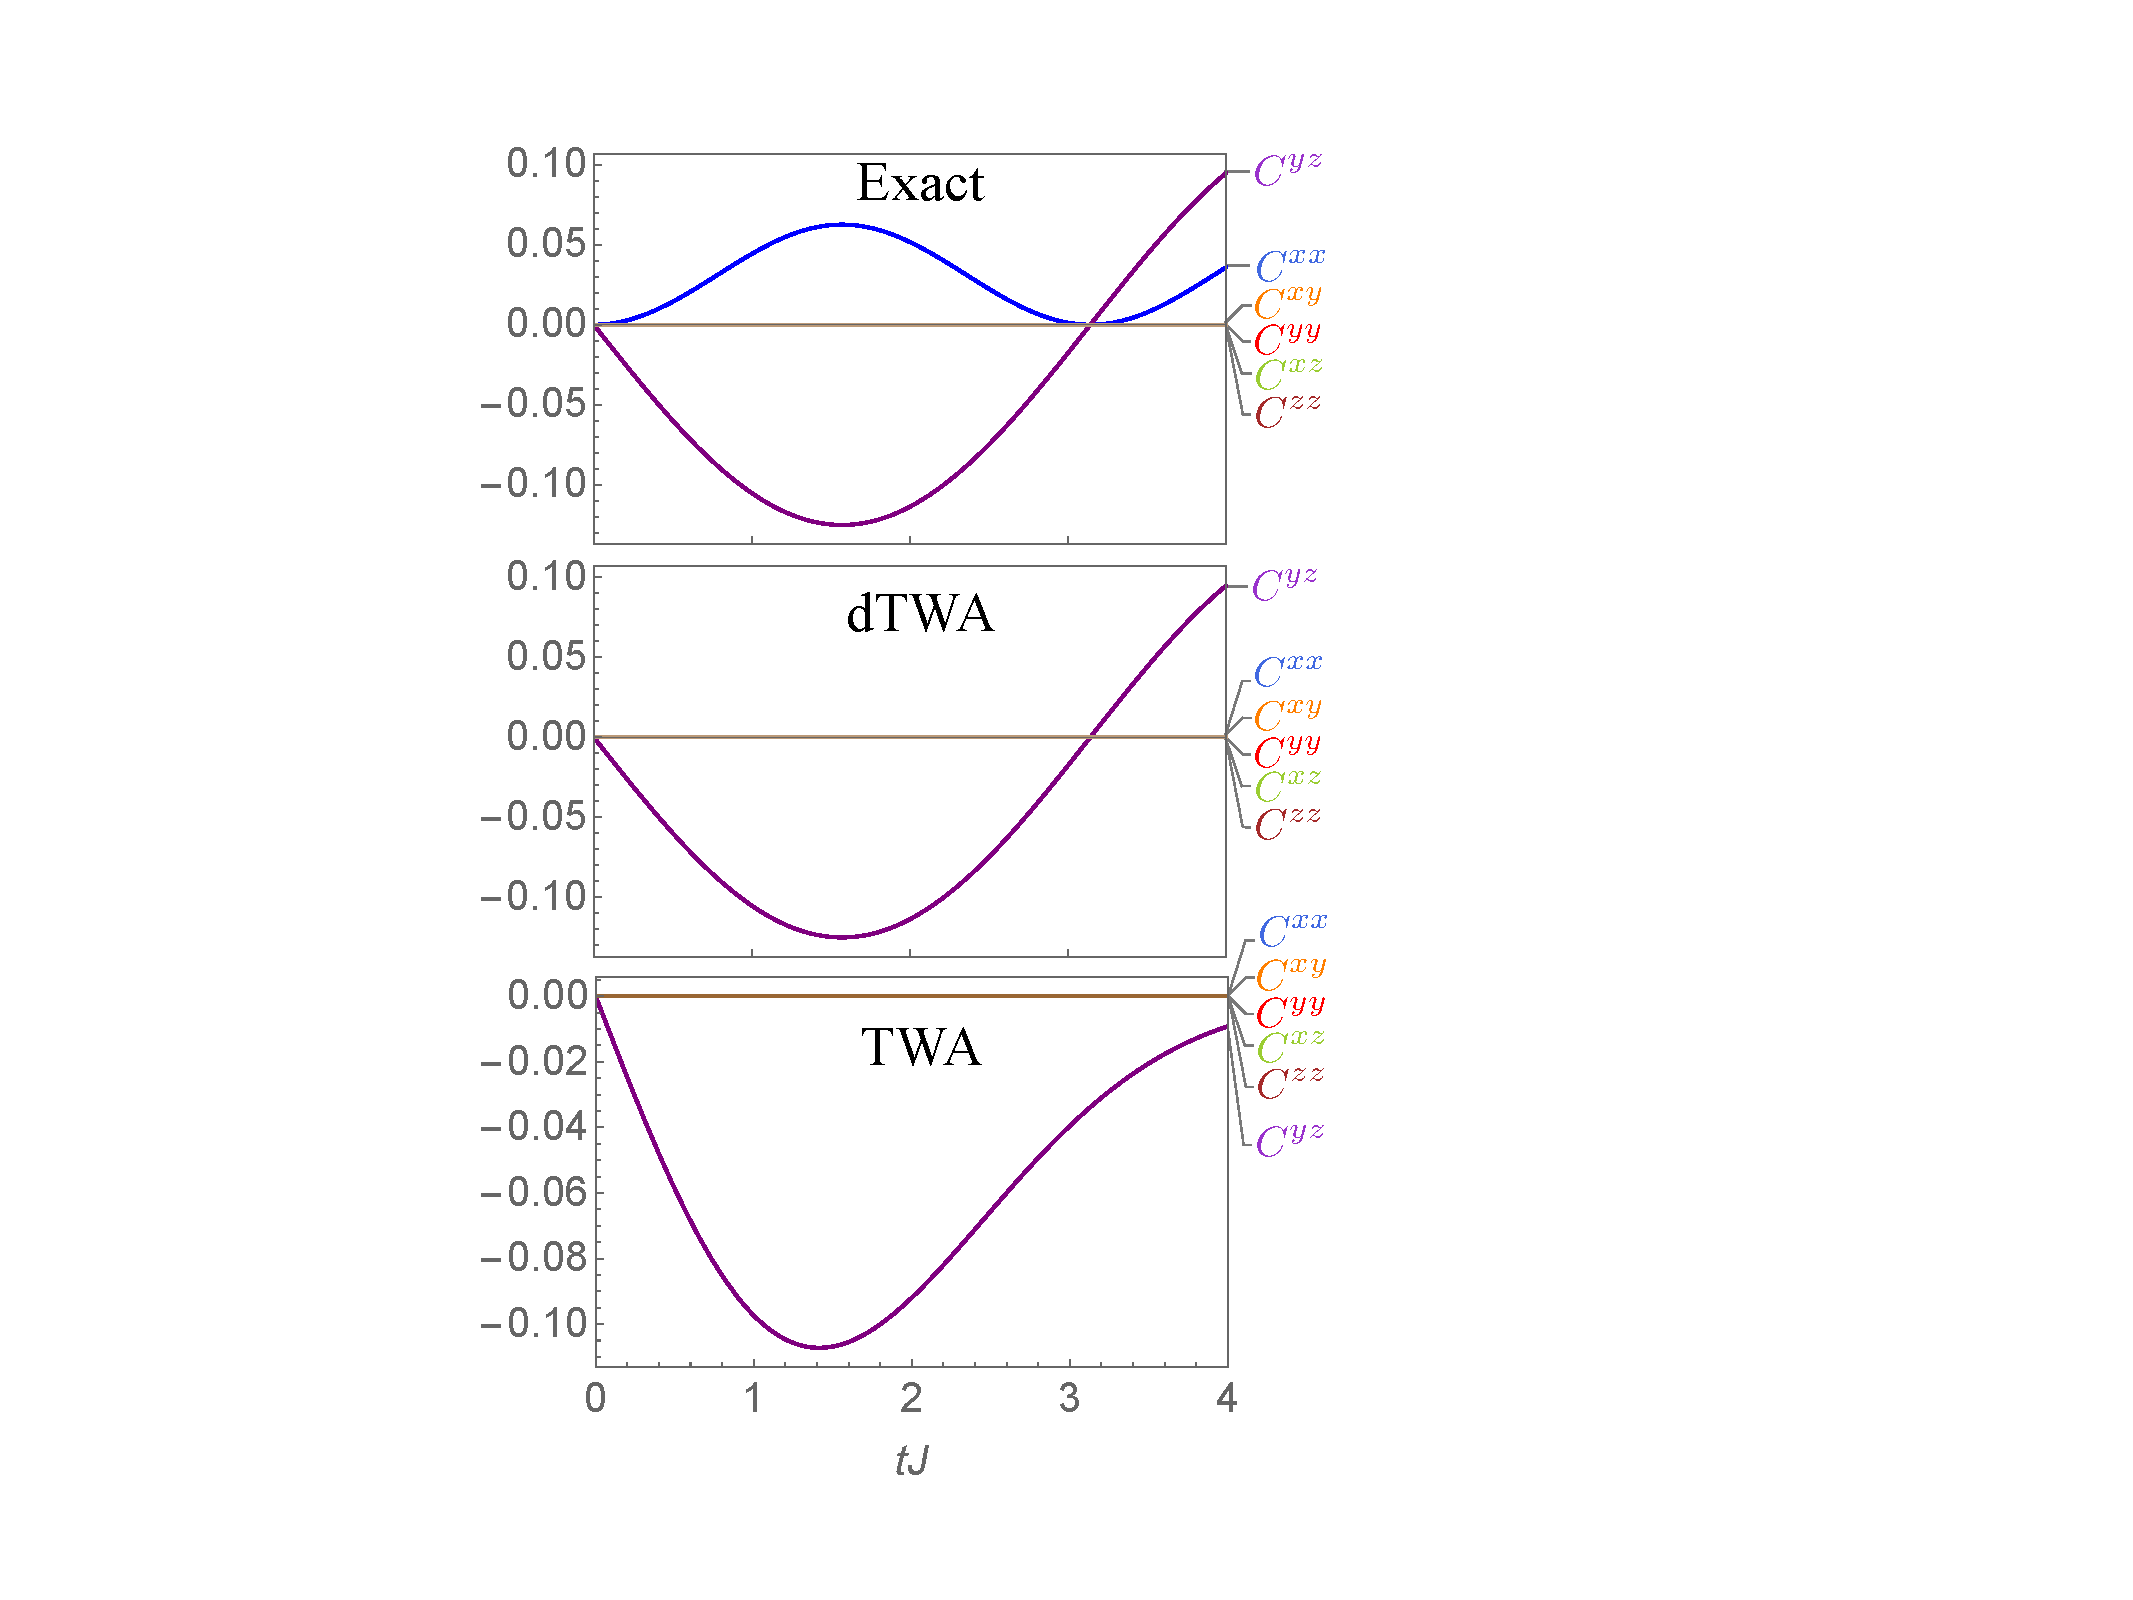
\includegraphics[width = 0.8\columnwidth]{fig8.pdf}
 \caption{(Color online) Components of correlation functions for a 1D Ising system ($h=0$) with spins initialized along the $\hat{x}$ direction.}
 \label{appendix1}
\end{figure}
\begin{figure}[t]\centering
 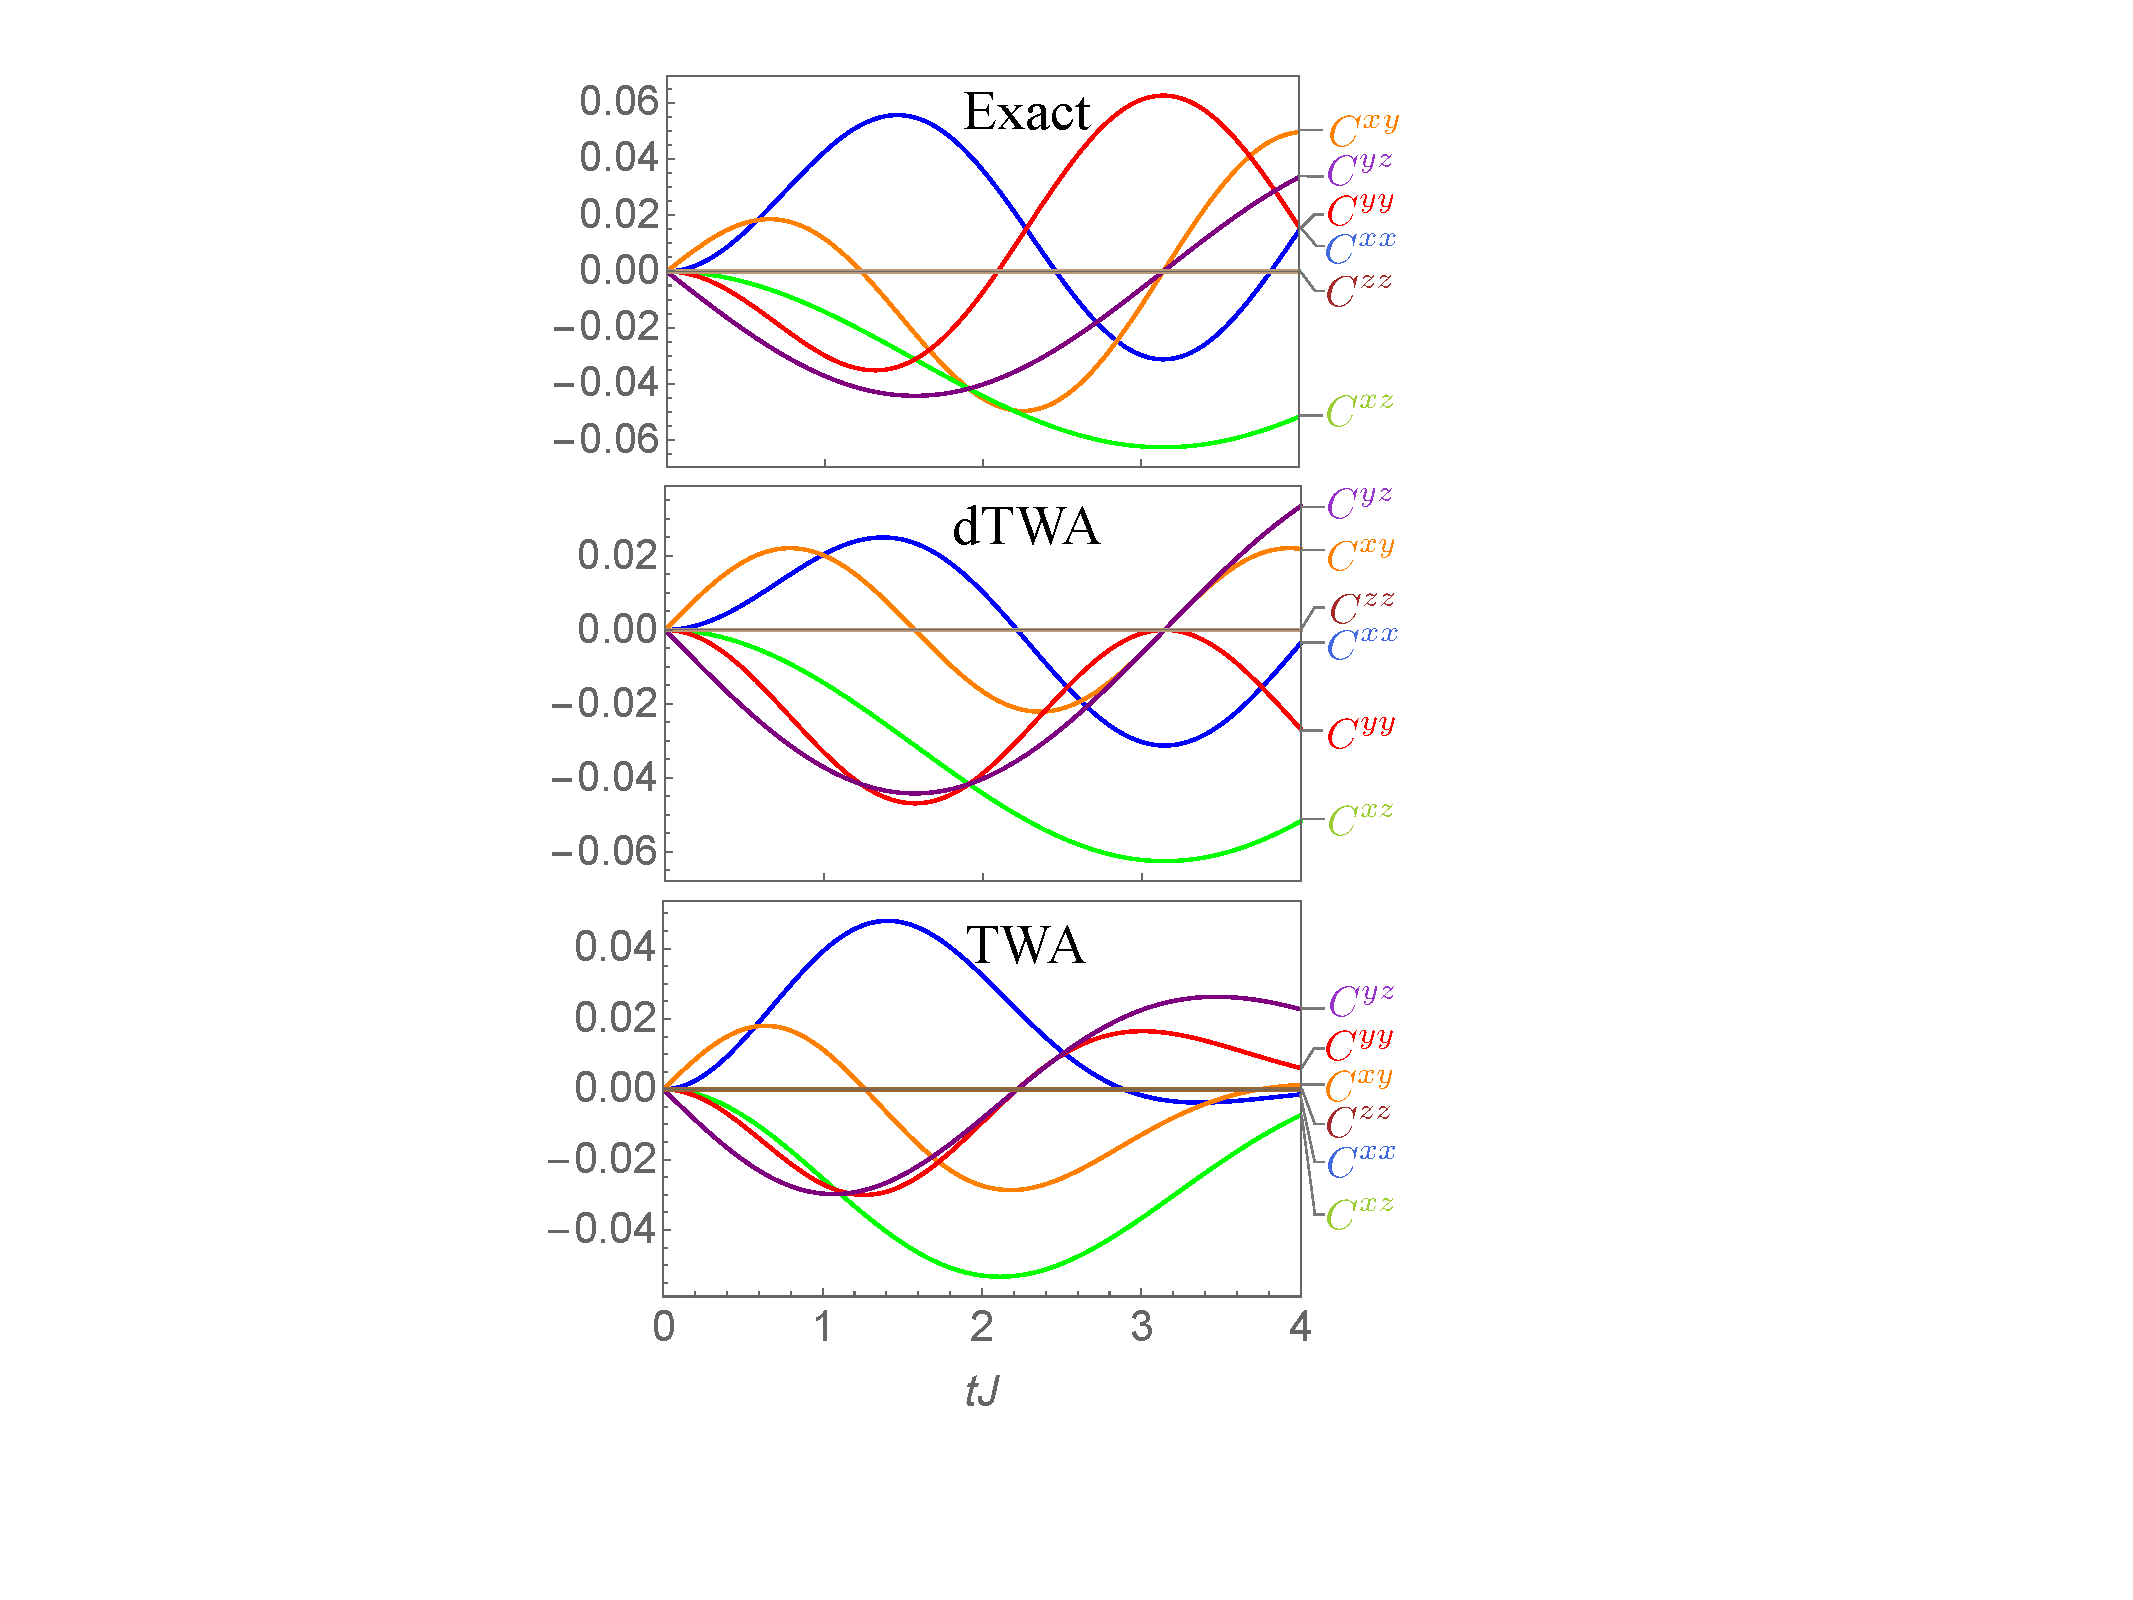
\includegraphics[width = 0.8\columnwidth]{fig9.pdf}
 \caption{(Color online) Components of correlation functions for a 1D Ising system ($h=0$) with spins initialized at $45^\circ$ between $\hat{x}$ and $\hat{z}$ on the $x$-$z$ plane.}
 \label{appendix2}
\end{figure}
\begin{figure}[t!]\centering
 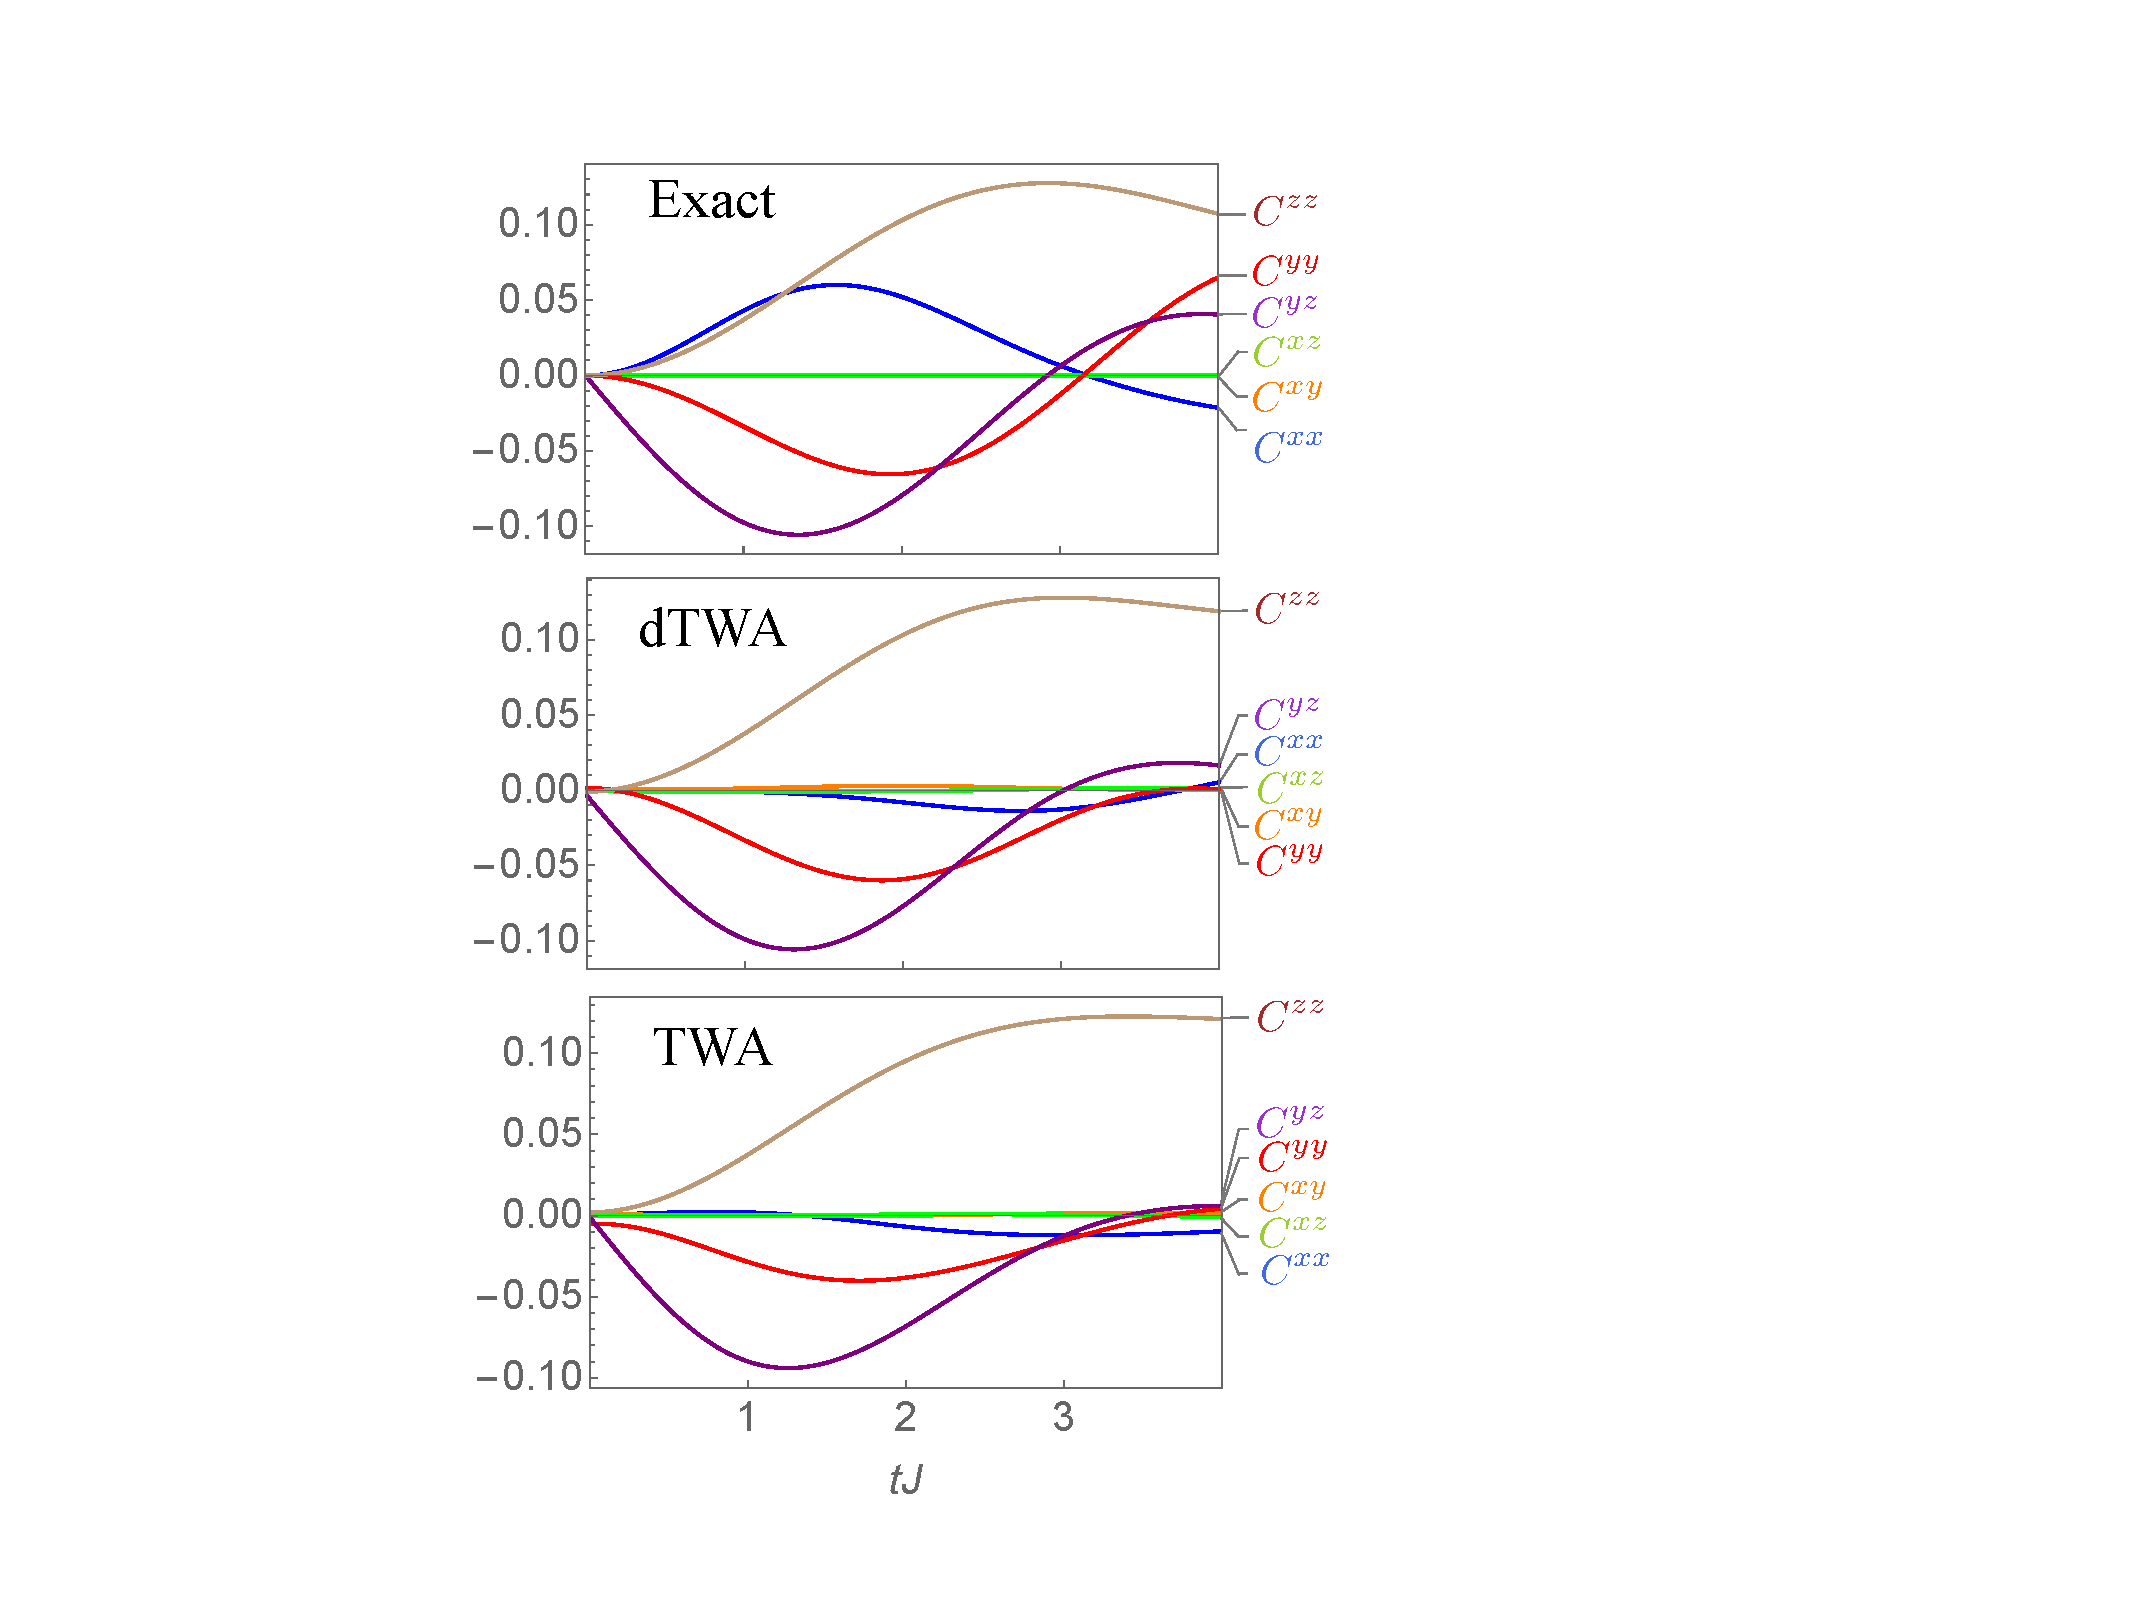
\includegraphics[width = 0.8\columnwidth]{fig10.pdf}
 \caption{(Color online) Components of correlation functions for a 1D Ising system ($h=J/3$) with spins initialized along the $\hat{x}$ direction.}
 \label{appendix3}
\end{figure}
\begin{figure}[h]\centering
 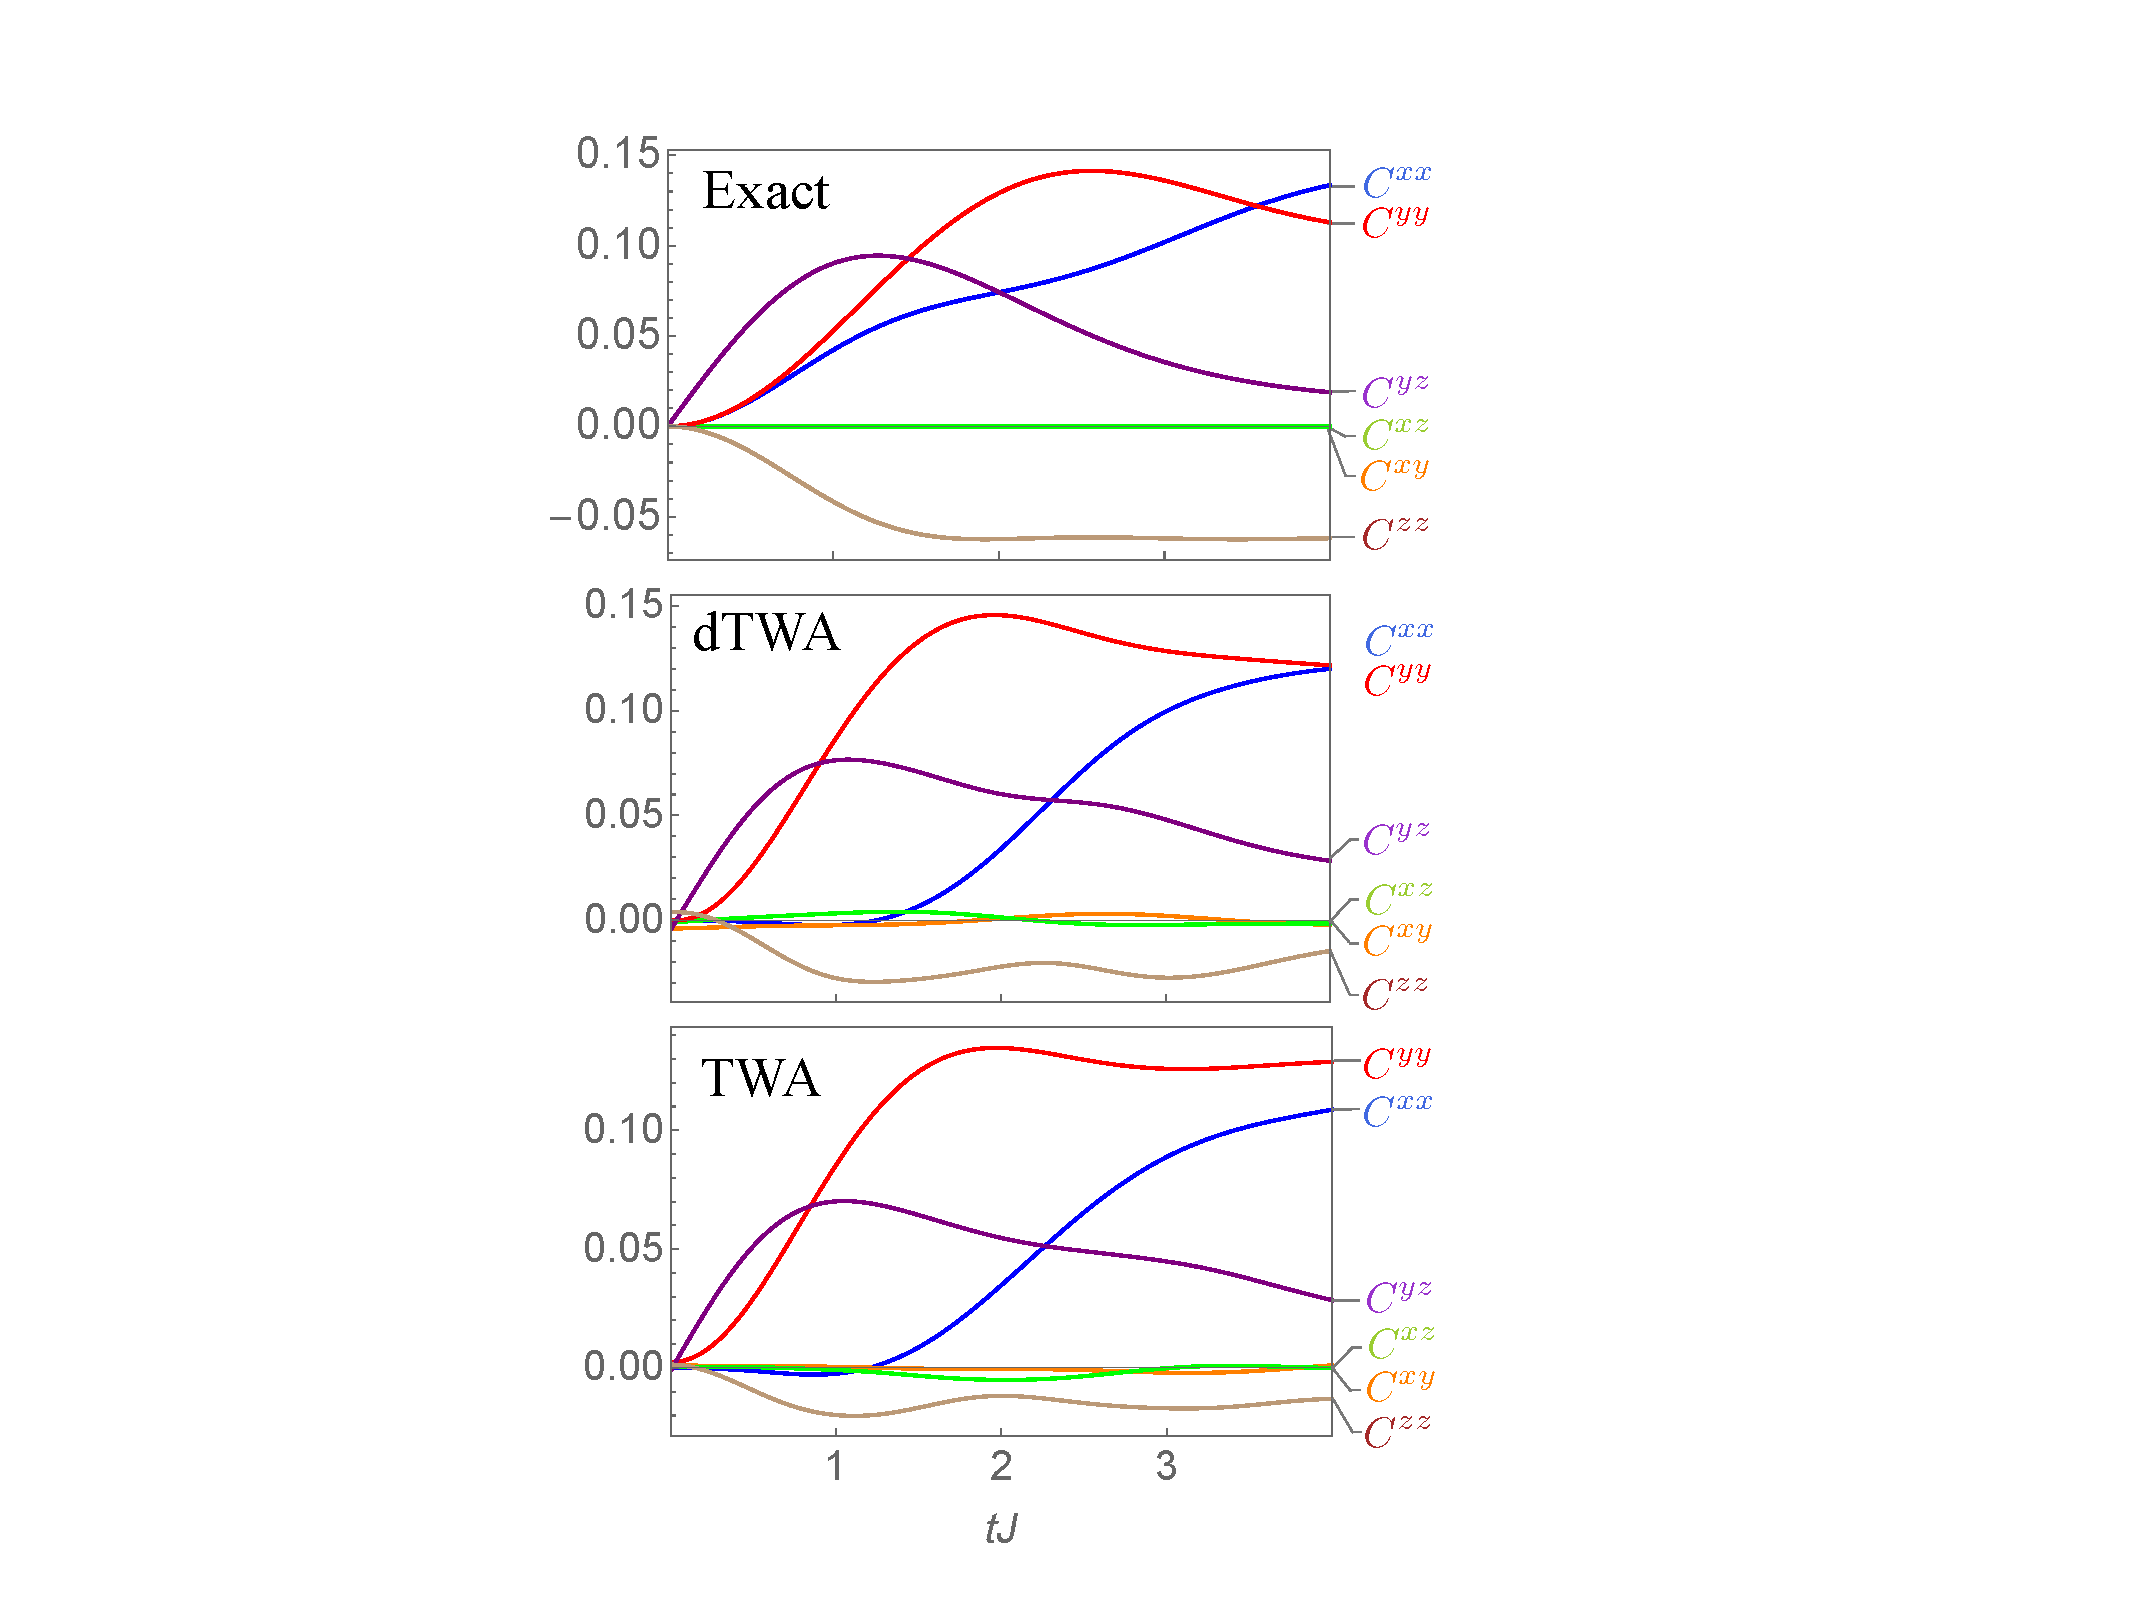
\includegraphics[width = 0.8\columnwidth]{fig11.pdf}
 \caption{(Color online) Components of correlation functions for a 1D XX system with spins initialized along the $\hat{x}$ direction..}
 \label{appendix4}
\end{figure}

\section*{Appendix A: Component-wise plots of spin correlations}\label{sec: component plots}
The main text compared TWA and dTWA with the exact solution using CMVs, in which several clear observations stood out. For example, the CMVs in the Wigner approximations had a ``two-dimensional" feature, and in some cases, the orientation of the CMV was reasonably correct up to moderate times only in TWA. This Appendix presents the same comparisons by conventional means, plotting each Cartesian component separately. Although this is the same information as presented in the main text, it is less clear from these plots, or sometimes even completely obscured, what information the Wigner approximations correctly capture or miss -- specifically simple trends such as the correlations along one direction being suppressed in all the Wigner approximations.

Figure~\ref{appendix1} plots all Cartesian components of the nearest-neighbor spin correlations for a system initialized in $\ket{\theta=\pi/2}$ and evolving under the 1D Ising model with no transverse field. For this case, it is clear that $C^{xx}$ is suppressed in both the Wigner approximations, because the suppressed component happens to be along a Cartesian direction.

In contrast, in Fig.~\ref{appendix2}, which plots plots all Cartesian components of the nearest-neighbor spin correlations for the initial state $\ket{\theta=\pi/4}$ evolving under the same 1D Ising model with no transverse field, the suppression of spin correlations along one direction is completely obscured, whereas this information is readily visible in Fig.~\ref{fig: Isingpi4}. This is because the component that is suppressed is not a Cartesian component, and moreover, the direction along which the CMV is squished rotates with time.

Figure~\ref{appendix3} plots all Cartesian components of the nearest-neighbor spin correlations for the initial state $\ket{\theta=\pi/2}$ evolving under the 1D transverse Ising model with $h=J/3$. It is clear that all Cartesian components besides $C^{zz}$ are smaller in both the Wigner approximations than the exact dynamics. However, other information readily visible in the CMVs in Fig.~\ref{fig: transIsing}, such as the direction along which the correlations are most suppressed, is not easily visible in Fig.~\ref{appendix3}.

Figure~\ref{appendix4} plots all components of the nearest-neighbor spin correlations for the initial state $\ket{\theta=\pi/2}$ evolving under the 1D XX model. In this figure as well, it is difficult to observe the suppression of correlations in the Wigner approximations, whereas this information is readily available in Fig.~\ref{fig: XX}

\section*{Appendix B: Analytical solutions for dynamics in the Ising model}\label{sec: analytical_expns}
Equations~\eqref{eqn: IsingEOM} for the 1D Ising model with no transverse field can be integrated to obtain analytical solutions for the exact and approximate dynamics of the Bloch vector $\smallexpect{\hat{\vec{S}}_i}$ and the spin-spin correlations $C_{ij}$. This Appendix sketches a derivation and lists the results for $\smallexpect{\hat{\vec{S}}_i}$ and $C_{ij}$ in the exact solution, dTWA, and TWA.

The solutions to the Ising equations of motion [Eq.~\eqref{eqn: IsingEOM}] are
\begin{equation}\label{eqn: IsingEOMSolns}
\left(\begin{array}{c}\hS^x_i(t)\\ \hS^y_i(t)\\ \hS^z_i(t)\end{array}\right) = \left(\begin{array}{ccc} \cos(\hB^z_it)&\sin(\hB^z_it)&0 \\ -\sin(\hB^z_it)&\cos(\hB^z_it)&0 \\ 0&0&1\end{array}\right)
\left(\begin{array}{c}\hS^x_i(0)\\ \hS^y_i(0)\\ \hS^z_i(0)\end{array}\right),
\end{equation}
where $\hB_i^\mu = J\left(\hS_{i-1}^\mu+\hS_{i+1}^\mu\right)$. From these, we can calculate the Bloch vector and spin-spin correlations. For example,
\begin{align}
\expect{\hat{S^x_i}}(t) = &\expect{\hS^x_i(0)\left(\cos^2\frac{Jt}{2}-4\hS^z_{i+1}(0)\hS^z_{i-1}(0)\sin^2\frac{Jt}{2}\right)}\nonumber\\ &+\expect{\hS^y_i(0)(\hS^z_{i+1}(0) + \hS^z_{i-1}(0))\sin(Jt)},
\end{align}
and this expression can be simplified further using translational symmetry and $\expect{\hS^y_i}(0)=0$ to
\begin{equation}
\expect{\hat{S^x_i}}(t) = \expect{\hS^x_i(0)}\left(\cos^2\frac{Jt}{2}-4\expect{\hS^z_i(0)}^2\sin^2\frac{Jt}{2}\right). \label{eqn: Sx exact}
\end{equation}
In the exact solution, this expression is evaluated by substituting the appropriate values for the initial conditions $\expect{\hS^\mu_i(0)}$. In the Wigner approximations, the quantum expectation $\langle\hat{O}\rangle$ is replaced by the initial average $\overline{\rm wl(\hat{O},\mathbf{S})}$ over the classical trajectories. Expressions for other Bloch vector and correlation components can be straightforwardly calculated in a similar manner to Eq.~\eqref{eqn: Sx exact}. We present only the results in the following sections. Exact solutions for the spin correlations in the 1D Ising model have also been calculated in Refs.~\cite{van2013relaxation, hazzard2014quantum}.

\newpage
\begin{widetext}
\subsection{Exact solution}
For a spin with initial wavefunction $\ket{\theta}$, the initial ensemble averages of spin operators are
\begin{align}\label{eqn: exact}
&\expect{\hS^x_j}(0) = \frac{1}{2}\sin\theta, \expect{\hS^y_j}(0) = 0, \expect{\hS^z_j}(0) = \frac{1}{2}\cos\theta,\nonumber\\
&\left(\hS^x_j\right)^2(0) = \left(\hS^y_j\right)^2(0) = \left(\hS^z_j\right)^2(0) = \frac{1}{4},\nonumber\\
&\expect{\hS^x_j\hS^y_j}(0) = -\expect{\hS^y_j\hS^x_j}(0) = \frac{i}{2}\cos\theta,\nonumber\\
&\expect{\hS^y_j\hS^z_j}(0) = -\expect{\hS^z_j\hS^y_j}(0) = \frac{i}{2}\sin\theta, \nonumber\\
&\expect{\hS^x_j\hS^z_j}(0) = \expect{\hS^z_j\hS^x_j}(0) = 0.
\end{align}
Using Eqs.~\eqref{eqn: IsingEOMSolns} and~\eqref{eqn: exact}, we obtain the magnetization and nearest-neighbor spin correlations at an arbitrary time as
\begin{align}
&\expect{\hat{\vec{S}}}_i(t) = \left(\frac{1}{2}\sin\theta\left(\cos^2\frac{Jt}{2}-\cos^2\theta\sin^2\frac{Jt}{2}\right), \frac{-1}{4}\sin(2\theta)\sin(Jt), \frac{1}{2}\cos\theta\right), \nonumber\\
&C^{xx}_{i,i+1}(t) = \frac{\sin^2\theta}{4} \left(\frac{\sin^2(Jt)}{4}(2+\cos2\theta)-\sin^4\frac{Jt}{2}\cos^4\theta\right),\nonumber\\
&C^{yy}_{i,i+1}(t) = -\frac{1}{16}\sin^22\theta\sin\frac{3Jt}{2}\sin\frac{Jt}{2},\nonumber\\
&C^{zz}_{i,i+1}(t) = 0, \nonumber\\
&C^{xy}_{i,i+1}(t) = C^{yx}_{i,i+1}(t) = \frac{1}{16}\sin\theta\sin2\theta\sin(Jt) \left(\cos(Jt)-2\cos^2\theta\sin^2\frac{Jt}{2}\right), \nonumber\\
&C^{xz}_{i,i+1}(t) = C^{zx}_{i,i+1}(t) = -\frac{1}{4}\sin^3\theta\cos\theta\sin^2\frac{Jt}{2},\nonumber\\
&C^{yz}_{i,i+1}(t) = C^{zy}_{i,i+1}(t) = -\frac{1}{8}\sin^3\theta\sin(Jt). \label{eqn: exactSoln}
\end{align}

\subsection{dTWA}
For a spin with initial wavefunction $\ket{\theta}$, the initial ensemble averages in dTWA over the classical trajectories are
\begin{align}\label{eqn: S8}
&\overline{S^x_j(0)} = \frac{1}{2}\sin\theta, \overline{S^y_j(0)} = 0, \overline{S^z_j(0)} = \frac{1}{2}\cos\theta,\nonumber\\
&\overline{\left(S^x_j\right)^2(0)} = \overline{\left(S^y_j\right)^2(0)} = \overline{\left(S^z_j\right)^2(0)} = \frac{1}{4},\nonumber\\
&\overline{S^\mu_jS^\nu_j(0)} = 0,\ \mu\neq\nu.
\end{align}
Using Eqs.~\eqref{eqn: IsingEOMSolns} and~\eqref{eqn: S8}, we obtain the magnetization and nearest-neighbor spin correlations at an arbitrary time as
\begin{align}
&\overline{\vec{S}_i(t)} = \left(\frac{1}{2}\sin\theta\left(\cos^2\frac{Jt}{2}-\cos^2\theta\sin^2\frac{Jt}{2}\right), \frac{-1}{4}\sin(2\theta)\sin(Jt), \frac{1}{2}\cos\theta\right), \nonumber\\
&C^{xx}_{i,i+1}(t) = \frac{\sin^22\theta}{16}\sin^2\frac{Jt}{2} \left(2\cos^2\frac{Jt}{2}-\cos^2\theta\sin^2\frac{Jt}{2}\right),\nonumber\\
&C^{yy}_{i,i+1}(t) = -\frac{3}{64}\sin^22\theta\sin^2(Jt),\nonumber\\
&C^{zz}_{i,i+1}(t) = 0, \nonumber\\
&C^{xy}_{i,i+1}(t) = C^{yx}_{i,i+1}(t) = \frac{1}{16}\sin\theta\sin2\theta\sin(Jt) \left(\cos^2\frac{Jt}{2}-2\cos^2\theta\sin^2\frac{Jt}{2}\right), \nonumber\\
&C^{xz}_{i,i+1}(t) = C^{zx}_{i,i+1}(t) = -\frac{1}{4}\sin^3\theta\cos\theta\sin^2\frac{Jt}{2},\nonumber\\
&C^{yz}_{i,i+1}(t) = C^{zy}_{i,i+1}(t) = -\frac{1}{8}\sin^3\theta\sin(Jt).
\end{align}
We find that the magnetization agrees with the exact solution at all times. Some components of the nearest-neighbor spin-spin correlations agree at all times, while others do only at short times. It is straightforward to show that one of the eigenvalues of the correlation matrix is always zero, and the corresponding eigenvector points along the direction $\left(1,-\cos\theta\tan\frac{Jt}{2}, \cot\theta(1-\sin^2\theta\sin^2\frac{Jt}{2}\right)$. As a result, the CMVs in this approximation are always ``two-dimensional''.

\subsection{TWA}
Finally, in TWA, the initial phase points for the wavefunction $\ket{\theta}$ are obtained by rotating the phase points sampled from the Wigner distribution associated with the state $\ket{\frac{\pi}{2}}$. Thus,
\begin{equation}\label{eqn: twa}
\overline{\vec{S}_i(0)} = \left(\begin{array}{ccc}\cos\theta&0&\sin\theta\\ 0&1&0\\ -\sin\theta&0&\cos\theta\end{array}\right) \left(\begin{array}{c}X_i/2\\ Y_i/2\\ 1/2\end{array}\right) 
= \frac{1}{2}\left( \sin\theta+X_i\cos\theta, Y_i, \cos\theta-X_i\sin\theta \right)^{\rm T},
\end{equation}
where $X_i$ and $Y_i$ are Gaussian random variables with mean $0$ and variance $1$. Using Eqs.~\eqref{eqn: IsingEOMSolns} and~\eqref{eqn: twa}, we obtain the magnetization and nearest-neighbor spin correlations at an arbitrary time as
\begin{align}
&\overline{\vec{S}_i(t)} = \left( \frac{1}{2}\sin\theta \cos(Jt\cos\theta)e^{-J^2t^2\sin^2\theta/4}, \frac{-1}{2}\sin(\theta) \sin(Jt\cos\theta)e^{-J^2t^2\sin^2\theta/4}, \frac{1}{2}\cos\theta \right),\nonumber\\
&C^{xx}_{i,i+1}(t) = \frac{Jt}{16}\sin2\theta\sin(Jt\cos\theta)e^{-J^2t^2\sin^2\theta/2} \left(\frac{Jt}{4}\sin2\theta\sin(Jt\cos\theta)+2\sin\theta\cos(Jt\cos\theta)\right),\nonumber\\
&C^{yy}_{i,i+1}(t) = \frac{Jt}{16}\sin2\theta\cos(Jt\cos\theta)e^{-J^2t^2\sin^2\theta/2} \left(\frac{Jt}{4}\sin2\theta\cos(Jt\cos\theta)-2\sin\theta\sin(Jt\cos\theta)\right),\nonumber\\
&C^{zz}_{i,i+1}(t) = 0, \nonumber\\
&C^{xy}_{i,i+1}(t) = C^{yx}_{i,i+1}(t) = \frac{Jt}{16}e^{-J^2t^2\sin^2\theta/2} \left(\sin\theta\sin2\theta\cos(2Jt\cos\theta) + \frac{Jt}{8}\sin^22\theta\sin(2Jt\cos\theta) \right), \nonumber\\
&C^{xz}_{i,i+1}(t) = C^{zx}_{i,i+1}(t) = -\frac{Jt}{8}\sin^3\theta\sin(Jt\cos\theta)e^{-J^2t^2\sin^2\theta/4},\nonumber\\
&C^{yz}_{i,i+1}(t) = C^{zy}_{i,i+1}(t) = -\frac{Jt}{8}\sin^3\theta\cos(Jt\cos\theta)e^{-J^2t^2\sin^2\theta/4}.
\end{align}
Unlike dTWA, the magnetization agrees with the exact solution only at short times. Moreover, clearly the magnetization and correlations exponentially decay with time, unlike the exact solutions and dTWA which undergo periodic oscillations. Additionally, it is straightforward to see that one of the eigenvalues of the correlation matrix in this approximation is also always zero, and the corresponding eigenvector points along the direction $\left(\cos(Jt\cos\theta), \sin(Jt\cos\theta), \cot\theta e^{-J^2t^2\sin^2\theta/4}\right)$.
\end{widetext}
\end{document}

